% concatenated from b_spline_paper.tex
\documentclass[10pt]{article}
\usepackage[margin=1in]{geometry}
\usepackage[utf8]{inputenc}
\usepackage{comment}
\usepackage{amsmath,amssymb,amsthm,amsfonts}
\newcommand{\dist}{\mathrm{dist}}
\newcommand{\supp}{\mathrm{supp}}
\renewcommand{\Re}{\mathrm{Re}\,}
\renewcommand{\Im}{\mathrm{Im}\,}
\newcommand{\Log}{\mathrm{Log\,}}
\newcommand{\floorn}{\lfloor \frac{n}{2}\rfloor}
\newcommand{\fracn}{\frac{n}{2}}
\usepackage{bbm}
\usepackage{tikz}
\usepackage{framed}
\usepackage{url}
\usepackage[backend=bibtex]{biblatex}
\nocite{*}
\addbibresource{refs.bib}
\usepackage{xcolor}
\pagecolor{white}
\usepackage{hyperref}

\newtheorem{theorem}{Theorem}[section]
\newtheorem{lemma}[theorem]{Lemma}
\newtheorem{corollary}[theorem]{Corollary}
%\theoremstyle{remark}

\theoremstyle{definition}
\newtheorem{definition}{Definition}[section]
\newtheorem*{remark}{Remark}


\numberwithin{equation}{section}
\numberwithin{figure}{section}
\numberwithin{table}{section}

\title{Rigorous High-Order Hausdorff Dimension Estimation of Limit Sets of Continued Fraction Iterated Function Systems via B-Splines}
\author{Jacob Brown\footnote{Department of Mathematics, University of Connecticut, Storrs, CT 06269, USA (e-mail: \href{mailto:jacob.l.brown@uconn.edu}{jacob.l.brown@uconn.edu)}}}
\date{\today}

\begin{document}

\maketitle

\begin{abstract}
We develop a method for the rigorous estimation of Hausdorff dimensions of limit sets produced by continued fraction iterated function systems. Our method is based on the approximation of a Perron-Frobenius operator using the finite element method with B-splines as the choice of basis functions. This choice provides key numerical advantages including higher-order convergence and computational flexibility. We prove an analogue of Falk and Nussbaum's result on ``hidden positivity" for B-spline quasi-interpolants to give rigorous upper and lower bounds for the Hausdorff dimensions of various limit sets. We provide numerical results to verify both the rigor and higher-order convergence of our method for quadratic B-spline interpolants in one and two dimensions.
\end{abstract}

\section{Introduction}

Recently, research interest in the fields of fractal geometry and dynamical systems has included the rigorous estimation of the Hausdorff dimensions of limit sets associated to iterated function systems. One of the earliest and most influential results is due to Hutchinson \cite{hutchinson1981fractals}: Let $X$ be a compact metric space and $\{\phi_e\}_{e=1}^m$ be a family of contractive similarities on $X$, with contraction ratios $r_e$, satisfying the open set condition. The Hausdorff dimension of the limit set is the parameter $s>0$ such that $\sum_{e=1}^mr_e^s=1$. This result is sometimes referred to as Hutchinson's formula. Using this formula, one can compute, for example, that the dimension of the $\frac{1}{3}$-Cantor Set is $\log2/\log3$, the dimension of the von Koch curve is $\log4/\log3$, and numerous other examples.

While powerful, Hutchinson's formula does not apply to systems with infinitely many maps, nor to systems whose maps do not consist of similarities. Many of these more complex systems are conformal iterated function systems (CIFSs). Mauldin and Urba\'{n}ski \cite{mauldin1996dimensions} employed the thermodynamic formalism to study these systems, and their methods set a theoretical framework for what would later allow numerical methods to be developed. In particular, they established that there is a unique parameter value $s>0$ such that the Perron-Frobenius operator (to be further discussed in Section 2)
$$L_sf(x)=\sum_{e\in E}\|D\phi_e(x)\|^sf(\phi_e(x))$$
has leading eigenvalue 1 with a strictly positive eigenfunction $f_s$, and that this parameter value is exactly equal to the Hausdorff dimension of the limit set of the CIFS. 

One particular CIFS that has garnered much interest is the \textit{continued fraction} CIFS. Any irrational number $x\in(0,1)$ can be expressed in continued fraction form,
$$x=[e_1(x),e_2(x),e_3(x),\dots]=\cfrac{1}{e_1(x)+\cfrac{1}{e_2(x)+\cfrac{1}{e_3(x)+\cfrac{1}{\dots}}}},\quad\quad e_i(x)\in\mathbb{N},\ i=1,2,\dots$$
There is a natural correspondence between these fractions and the CIFS consisting of $[0,1]$ and the maps
$$\phi_e(x)=\frac{1}{x+e},\quad e\in \mathbb{N}.$$
In particular, for any subset $E\subset\mathbb{N}$ the limit set associate to the system restricted to the maps $\{\phi_e:e\in E\}$ is precisely the set of irrational numbers whose continued fraction expansion only contains elements in $E$. Rigorous dimension estimates for various choices of $E$ has been the subject of numerous publications in recent years. Notably, Pollicott and Vytnova were able to estimate the dimension of the limit set associate to $E=\{1,2\}$ to an accuracy of 200 digits \cite{pollicott2022hausdorff}.

In light of the result of Mauldin and Urba\'{n}ski, numerical methods for approximating the Perron-Frobenius operator and, in turn, the Hausdorff dimensions of various limit sets of CIFSs—and the continued fraction CIFS in particular—were developed. Recently, Falk and Nussbaum developed and iterated upon an approach to approximate the Perron-Frobenius operator using a collocation method based on continuous piecewise multilinear functions \cite{falk2018new,falk2018c}, and subsequently based on continuous piecewise polynomials of arbitrary degree \cite{falk2021hidden}. Their method was employed by Chousionis et al. \cite{chousionis2020dimension} to study the dimension spectra of subsystems of the continued fraction CIFS. Chousionis et al. \cite{chousionis2024rigorous} further developed a finite element method approach using piecewise linear polynomials to obtain rigorous dimension estimates for higher-dimensional continued fractions, the Apollonian gasket, and other systems.

A common obstacle in these numerical methods is the need for positivity preservation in the approximation scheme, which is necessary to obtain rigorous estimates. A result of Korovkin states that any linear approximation scheme that preserves positivity must be at most second-order accurate \cite{korovkin1957order}. Commonly, the Perron-Frobenius operator is approximated by a matrix, and this matrix needs to have nonnegative entries in order for a theorem regarding the spectral radius of positive matrices to hold (See Lemma \ref{lem:pos_mat} in Section 2). 

In \cite{falk2021hidden}, Falk and Nussbaum circumvented the need for positivity in the traditional sense by showing that the Perron-Frobenius operator maps a certain cone of functions into itself, which allowed them to utilize an extension of Lemma \ref{lem:pos_mat}. Through this extension, they were able to utilize polynomial interpolants of degree greater than 1, which do not necessarily preserve positivity and thus lead to negative entries in the approximation matrices. They coined the term ``hidden positivity" to refer to this more abstract notion of positivity.

One technical difficulty encountered by the authors was that in order for their results to hold, they needed to employ approximations of an iterated operator,
$$L^\nu_sf(x)=\sum_{e\in E^\nu}\|D\phi_e(x)\|^sf(\phi_e(x)).$$
While this iterated operator has a smaller domain requiring fewer mesh points to approximate, the increase in the number of terms in the alphabet usually offsets any computational advantages. The authors noted, however, that they found no cases where their method failed if they did not iterate the operator, leading them to conjecture that this condition was only an artifact of the method of proof.

In this paper, we consider a finite element method approach to estimate the Hausdorff dimensions of continued fraction CIFSs based on B-splines. As we will show, our method has several key advantages. We show that quasi-interpolation of $L_s$ using B-splines of degree $n$ results in convergence of order $n+1$, which allows us to obtain rigorous estimates without turning to high-degree interpolants. Moreover, we resolve the conjecture of Falk and Nussbaum by showing that neither the proof nor the implementation of this method requires iteration on the alphabet. Finally, we show that our hidden positivity result extends to B-spline interpolants in all dimensions, allowing us to rigorously estimate dimensions of higher-dimensional systems.

The rest of the paper is structured as follows. In Section 2 we provide background information for B-splines, conformal iterated function systems, and Falk and Nussbaum's hidden positivity. We also prove some technical results (Theorems \ref{thm:partial_est} and \ref{thm:third_bounds}). In Section 3 we prove our main theoretical results on hidden positivity for B-splines in both one dimension and higher dimensions. Finally, in Section 4 we provide numerical examples of rigorous upper and lower dimension estimates for various alphabets in one and two dimensions using quadratic B-splines as our basis functions. We also provide calculations to show that our method converges with order 3, in accordance with our theoretical results.
%We describe the theory underlying the approximation as well as the advantages to using B-splines over other approximation methods. Moreover, we show that Falk and Nussbaum's notion of hidden positivity holds for B-spline approximations of arbitrary degree and dimension. This is necessary because, as described in Section 2, the approximation obtained using B-splines of degree greater than 1 are not necessarily positivity-preserving. Finally, we present numerical results for various continued fraction systems in one and two dimensions.

\section{Preliminaries}

In this section we introduce the necessary background about B-splines and the continued fraction conformal iterated function system. 

\subsection{B-Splines}

We adopt the algorithmic point of view for B-splines presented by de Boor and H\"{o}llig and discussed in \cite{hollig2013approximation}, as opposed to the more traditional definition via divided differences.

\begin{definition}
A \textit{knot sequence} $\xi=\{\xi_k\}_{k\in I}$ is a finite or bi-infinite non-decreasing sequence of real numbers (called \textit{knots}) without accumulation points, where $I$ denotes the index multi-set of the knot sequence. The number of times a knot $\xi_k$ appears in the sequence is called its \textit{multiplicity}, which is denoted by $\#\xi_k$, and if $\#\xi_k\geq2$, we refer to $\xi_k$ as a \textit{repeated knot}. The knot sequence partitions a subset $R\subseteq\mathbb{R}$ into \textit{knot intervals} $[\xi_\ell,\xi_{\ell+1})$. A knot sequence is \textit{uniform} if all of its knot intervals have equal length.
\end{definition}

Figure \ref{fig:knot_sequence} shows an example of a knot sequence. The use of the index $\ell$ for the knot intervals comes from the fact that intervals of the form $[\xi_k,\xi_{k+1})$ can be degenerate in the case when the knot sequence has repeated knots. If the knot sequence has no repeated knots, then the indices $\ell$ and $k$ coincide, in which case we will write $[\xi_k,\xi_{k+1})$ to denote the knot intervals.

\begin{figure}[b]
\centering
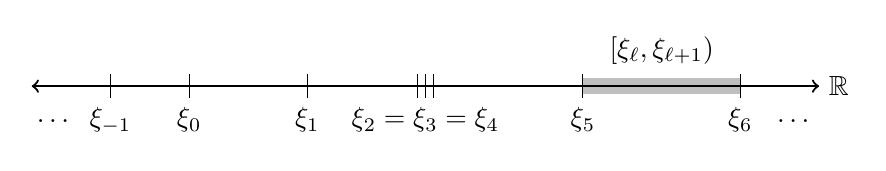
\begin{tikzpicture}
            \fill[gray!50] (7,-0.1) rectangle (9,0.1);
            \draw[<->, thick] (0,0)--(10,0);
            \draw (1,0.15)--(1,-0.15);
            \draw (2,0.15)--(2,-0.15);
            \draw (3.5,0.15)--(3.5,-0.15);
            \draw (5,0.15)--(5,-0.15);
            \draw (5.1,0.15)--(5.1,-0.15);
            \draw (4.9,0.15)--(4.9,-0.15);
            \draw (7,0.15)--(7,-0.15);
            \draw (9,0.15)--(9,-0.15);
            
            \node[anchor=south] at (8,0.15) {$[\xi_{\ell},\xi_{\ell+1})$};
            \node[anchor=north] at (0.3,-0.3) {$\dots$};
            \node[anchor=north] at (9.7,-0.3) {$\dots$};
            \node[anchor=north] at (1,-0.15) {$\xi_{-1}$};
            \node[anchor=north] at (2,-0.15) {$\xi_0$};
            \node[anchor=north] at (3.5,-0.15) {$\xi_1$};
            \node[anchor=north] at (7,-0.15) {$\xi_5$};
            \node[anchor=north] at (9,-0.15) {$\xi_6$};
            \node[anchor=north] at (5,-0.15) {$\xi_2=\xi_3=\xi_4$};
            \node[anchor=west] at (10,0) {$\mathbb{R}$};
        \end{tikzpicture}
        \caption{An example of a knot sequence.}
\label{fig:knot_sequence}

\end{figure}

\begin{definition}
Given a knot sequence $\xi=\{\xi_k\}_{k\in I}$, we define the degree $n$ \textit{B-splines} using the following recurrence relation. The degree 0 B-splines are defined as the characteristic functions of the knot intervals,
$$b^0_{k,\xi}(x)=\begin{cases}
1&\text{if $\xi_k\leq x<\xi_{k+1}$}\\
0&\text{otherwise.}
\end{cases}$$
The degree $n$ B-splines for $n\geq 1$ are defined inductively as
$$b^n_{k,\xi}=\gamma^n_{k,\xi}b^{n-1}_{k,\xi}+(1-\gamma^n_{k+1,\xi})b^{n-1}_{k+1,\xi},\quad\text{where }\gamma^n_{k,\xi}(x)=\frac{x-\xi_k}{\xi_{k+n}-\xi_k}.$$
For knot sequences with repeated knots, we discard any terms where the denominator of $\gamma^n_{k,\xi}$ vanishes. It can be shown that the derivative of a B-spline follows the recursion
\begin{equation}
(b^n_{k,\xi})'=\alpha_{k,\xi}^nb^{n-1}_{k,\xi}-\alpha_{k+1,\xi}^{n}b^{n-1}_{k+1,\xi},\quad\text{where }\alpha^n_{k,\xi}=\frac{n}{\xi_{k+n}-\xi_{k}}.
\label{eqn:bsplinederiv}
\end{equation}
\end{definition}

The \textit{parameter interval} $D^n_\xi$ of the B-splines $b^n_{k,\xi}$ is the maximal interval on which the collection of $b^n_{k,\xi}$ form a partition of unity. Figure \ref{fig:param_int} shows an example of a collection of quadratic B-splines and their parameter interval. As can be seen, the parameter interval is a proper subinterval of the entire domain on which the B-splines are constructed. In particular, for degree $n$ B-splines on a finite knot sequence without repeated knots, the parameter interval is obtained by removing $n$ leftmost and $n$ rightmost knot intervals. We require that the parameter interval span the entire domain of the function to be approximated in order for the upcoming approximation results to hold. As such, in implementation, we will need to expand our computational domain by $n$ knot intervals on each side. 

\begin{figure}
\centering
\includegraphics[width=0.5\linewidth]{quad_splines_param_tex}
\caption{The parameter interval $D^2_\xi=[2,5]$ when using quadratic B-splines on the domain $[0,7]$ with knot sequence $\xi=\{0,1,2,\dots,7\}$.}
\label{fig:param_int}
\end{figure}

It follows immediately from the definition that $b^n_{k,\xi}$ is non-negative for all $n$. For our discussion, we will assume that the knot sequence has no repeated knots. Under this assumption, the support of the B-spline is $\supp(b^n_{k,\xi})=[\xi_k,\xi_{k+n+1}]$, that is, the closure of $n+1$ consecutive knot intervals. When the degree and knot sequence are clear, we will write $b_k$ to ease the notation. Given a point $x$, we write $k\sim x$ to denote the B-splines ``relevant" to $x$, i.e., $k\sim x=\{k:b_k(x)>0\}$, and for a set $\Omega$ we write $k\sim\Omega$ to denote the B-splines such that $k\sim x$ for some $x\in\Omega$.

%The parameter interval of degree $n$ B-splines defined on a finite knot sequence $\xi=\{\xi_0,\xi_1,\dots,\xi_m\}$ without repeated knots and where $m\geq 2n$ is $[\xi_n,\xi_{m-n}]$. This fact will be of consequence for the construction of our approximations.

The construction of a $d$-dimensional B-spline is rather straightforward, as it is simply the tensor product of one-dimensional B-splines. To be precise, we first equip each axis $j=1,2,\dots,d$ with a knot sequence $\xi_j=\{\xi_{k_j}\}_{k_j\in I_j}$, where $I_j$ is the index set corresponding to axis $j$. We then construct the degree $n_j$ B-splines $b_{k_j,\xi_j}^{n_j}$ along each axis, and define the $d$-dimensional B-spline as
$$b_{k,\xi}^n(x_1,x_2,\dots,x_d)=\prod_{j=1}^db_{k_j,\xi_j}^{n_j}(x_j),$$
where $n=(n_1,n_2,\dots,n_d)$ is the so-called coordinate degree of the $d$-dimensional B-spline.

As in the univariate case, there is a subset $D^n_\xi$ of the domain on which the collection of B-splines forms a partition of unity, called the \textit{parameter (hyper)rectangle}. Figure \ref{fig:param_int_2d} shows an example of the parameter rectangle for quadratic B-splines in $\mathbb{R}^2$.

\begin{figure}[b]
\centering
\includegraphics[width=0.5\linewidth]{2d_param_int}
\caption{Example of the parameter rectangle for 2-dimensional B-splines.}
\label{fig:param_int_2d}
\end{figure}

\clearpage
We now turn our attention to approximation using B-splines.
\begin{definition}
Let $\{b_k\}$ be the collection of degree $n$ B-splines defined on a knot sequence $\xi$ with parameter interval $D^n_\xi$. A linear B-spline approximation scheme of the form $f\approx Qf=\sum_k (Q_kf)b_k$ is called a \textit{quasi-interpolant} provided
\begin{enumerate}
\item Each $Q_k$ is a linear functional that acts on $f$.
\item Each $Q_k$ is locally bounded. That is, there is a number $\|Q\|>0$ such that 
$$|Q_kf|\leq \|Q\|\,\|f\|_{\infty,[\xi_k,\xi_{k+n+1}]}$$
for each $Q_k$, where $\|f\|_{\infty,U}=\sup\{|f(x)|:x\in U\}$.
\item $Qp(x)=p(x)$ for every $x\in D^n_\xi$ and polynomial $p$ of degree at most $n$.
\end{enumerate}
\end{definition}

Quasi-interpolants are desirable for their accuracy in approximating functions and their derivatives, as shown in the following result whose proof can be found on page 86 of \cite{hollig2013approximation}.

\begin{theorem}
\label{thm:quasi_error}
Let $f$ be $n+1$ times continuously differentiable and $Qf=\sum_k(Q_kf)b_k$ be a quasi-interpolant of $f$ using degree $n$ B-splines on a knot interval $\xi$ with parameter interval $D^n_\xi$. For each $x\in D^n_\xi$, let $D_x=\bigcup_{k\sim x}\supp(b_k)$ and $h(x)=\max\{|x-y|:y\in D_x\}$. Then
$$|f(x)-Qf(x)|\leq \frac{\|Q\|}{(n+1)!}\|f^{(n+1)}\|_{\infty,D_x}h(x)^{n+1}.$$
Further suppose that the quotients of consecutive knot intervals are uniformly bounded by $r$. Then for all $1\leq j\leq n$, there is a constant $C$ depending on $n$ and $r$ such that
$$|f^{(j)}(x)-(Qf)^{(j)}(x)|\leq C\|Q\|\|f^{(n+1)}\|_{\infty,D_x}h(x)^{n+1-j}.$$
\end{theorem}

We will be using uniform meshes in all of our computational examples. Therefore, if the mesh size is $h$, since $x$ lies in the middlemost interval of $2n+1$ consecutive knot intervals, we have $h(x)\leq(n+1)h$. Replacing $\|f^{(n+1)}\|_{\infty,D_x}\leq\|f^{(n+1)}\|_\infty$, we have the estimates
$$|f(x)-Qf(x)|\leq \frac{(n+1)^{n+1}\|Q\|}{(n+1)!}\|f^{(n+1)}\|_{\infty}h^{n+1}=\frac{(n+1)^n\|Q\|}{n!}\|f^{(n+1)}\|_{\infty}h^{n+1}$$
and 
$$|f^{(j)}(x)-(Qf)^{(j)}(x)|\leq \frac{2n(n+1)^{n+1-j}\|Q\|}{(n+1)!}\|f^{(n+1)}\|_{\infty}h^{n+1-j}=\frac{2(n+1)^{n-j}\|Q\|}{(n-1)!}\|f^{(n+1)}\|_{\infty}h^{n+1-j}.$$

As we will see in the coming sections, there are conditions on how small $h$ must be chosen in order for our numerical results to be rigorous. Therefore, we require explicit formulas and/or estimates for every constant in the inequalities above. In particular, we need to be able to compute $\|Q\|$, the boundedness constant of the quasi-interpolant. Below, we will describe our construction of the quasi-interpolant and list the value of $\|Q\|$ for various degrees of the quasi-interpolant. Estimates for $\|f^{(n+1)}\|_{\infty}$ and the other derivatives will be presented in the next subsection.%This number depends on the sample points used 

On a uniform knot sequence with grid size $h$, a natural choice for the quasi-interpolant linear functionals is a weighted sum of the function values at the midpoints of the knot intervals on which $b_k$ is supported. That is,
$$Q_kf=\sum_{v=0}^nw_vf(\xi_{k+v}+h/2),$$
where the weights $w_v$ satisfy the linear system
$$\sum_{v=0}^nw_v(v-j)^n=\prod_{i=1}^n(i-j-1/2).$$
Some important properties of these weights are: (i) $\sum_{v=0}^nw_v=1$, (ii) $w_{\lfloor\frac{n}{2}\rfloor}=\max_v|w_v|$, and (iii) $w_v=w_{n-v}$ for $v=0,1\dots,n$. We remark that a choice for $\|Q\|$ that satisfies the local boundedness requirement for this choice of quasi-interpolant is $\|Q\|=\sum_{v=0}^n|w_v|$. In Table \ref{table:weights}, we provide the weights and the value of $\|Q\|$ for this construction of the quasi-interpolant for $n=1,2,3,$ and $4$.

\begin{table}[h]
\centering
\begin{tabular}{c|c|c|c|c|c|c}
& $w_0$ & $w_1$ & $w_2$ & $w_3$ & $w_4$ & $\|Q\|$ \\\hline
$n=1$ & $1/2$ & $1/2$ & & & & $1$ \\\hline
$n=2$ & $-1/8$ & $5/4$ & $-1/8$ & & & $3/2$ \\\hline
$n=3$ & $-7/48$ & $31/48$ & $31/48$ & $-7/48$ & & $19/12$   \\\hline
$n=4$ & $47/1152$ & $-107/288$ & $319/192$ & $-107/288$ & $47/1152$  & $179/72$ \\
\end{tabular}
\caption{Weights for the 1D quasi-interpolant using the midpoints of the knot intervals for $n=1,2,3,4$ \cite{hollig2013approximation}.}
\label{table:weights}
\end{table}



The generalization of quasi-interpolants to $\mathbb{R}^d$ proceeds similarly to the generalization of B-splines to higher dimensions. We assume that each axis has been equipped with a uniform knot sequence $\xi_j$ with grid size $h_j$. Let $w_{v_j}$, $v_j=0,1,\dots,n_j$ be the weights corresponding to the one-dimensional quasi-interpolant on axis $j$, then the $d$-dimensional quasi-interpolant is defined as $f\approx Qf=\sum_k(Q_kf)b_k$, where the $b_k$ are the $d$-dimensional B-splines and 
\begin{align*}
Q_kf&=Q_{(k_1,k_2,\dots,k_d)}f\\
&=\sum_{v_1=0}^{n_1}\sum_{v_2=0}^{n_2}\cdots\sum_{v_j=0}^{n_j}w_{v_1}w_{v_2}\cdots w_{v_d}f(\xi_{k_1+v_1}+h_1/2,\xi_{k_2+v_2}+h_2/2,\dots,\xi_{k_d+v_d}+h_d/2).
%\label{eqn:d_dim_quasi}
\end{align*}

That is, the coefficient $Q_kf$ is a weighted sum of the function values at the midpoints of the hyperrectangles on which $b_k$ is supported, and the weight on each midpoint is the product of the weights in the one-dimensional quasi-interpolant. As with the univariate case, there is an approximation result for higher-dimensional quasi-interpolants. In order to state this result, we need the following bound on polynomial approximation. We provide the statement as written in \cite{hollig2013approximation}---since we will make a slight modification to it---but the original result is due to Reif \cite{reif2012polynomial}.
\begin{theorem}
\label{thm:poly_bound}
For a hyperrectangle $R=[a_1,b_1]\times\dots\times[a_d,b_d]$, let $\mathbb{P}^n(R)$ denote the space of polynomials of degree at most $n$ on $R$. For a function $f$ on $R$, the error of the orthogonal projection $P^nf\in\mathbb{P}^n(R)$ defined by
$$\int_Rfq\,dx=\int_R(P^nf)q\,dx\quad\text{for all $q\in\mathbb{P}^n(R)$}$$
is bounded by
$$|f(x)-P^nf(x)|\leq c(n,d)\sum_{v=1}^dh_v^{n+1}\|\partial_v^{n+1}f\|_{\infty,R},$$
where $h_v$ is the width of $R$ in the $v$-th direction and $c(n,d)$ is a constant depending on $n$ and $d$.
\end{theorem}

We will now compute the constant $c(n,d)$ following the proof \cite{hollig2013approximation}, but we will make an adjustment that yields a better constant. First, we note that the estimate is invariant under translation and dilation, and thus we may take $R=[0,1]^d$. Let $p_0,p_1,\dots,p_n$ be an orthonormal basis for $\mathbb{P}^n([0,1])$, then by the boundedness of an orthogonal projection we have $\|P^nf\|_{\infty,[0,1]}\leq c_1(n)\|f\|_{\infty,[0,1]}$ where
\begin{equation}
c_1(n)=\sum_{k=0}^n\left(\int_0^1|p_k|\,dx\right)\|p_k\|_{\infty,[0,1]}.
\label{eq:c_1}
\end{equation}
Then for any $p\in \mathbb{P}^n([0,1])$, we have
$$\|f-P^nf\|_{\infty,[0,1]}\leq\|f-p\|_{\infty,[0,1]}+\|P^n(f-p)\|_{\infty,[0,1]}\leq(1+c_1(n))\|f-p\|_{\infty,[0,1]}.$$
By choosing $p$ to be the Taylor polynomial to $f$ at $x=1/2$, we obtain 
$$\|f-p\|_{\infty,[0,1]}\leq \frac{1}{2^n(n+1)!}\|f^{(n+1)}\|_{\infty,[0,1]}.$$
Thus, $\|f-P^nf\|_{\infty,[0,1]}\leq c_2(n)\|f^{(n+1)}\|$ with
\begin{equation}
c_2(n)=\frac{1+c_1(n)}{2^n(n+1)!}.
\label{eq:c_2}
\end{equation}
We refer the reader to \cite{hollig2013approximation} for the remainder of the proof. The constant $c(n,d)$ is given by
\begin{equation}
c(n,d)=c_2(n)\sum_{v=1}^dc_1(n)^{v-1}=\frac{c_2(n)[1-c_1(n)^{d}]}{1-c_1(n)}
\label{eq:multi_error_bound}
\end{equation}

With this result stated, we can now state the error bound for multidimensional quasi-interpolants (see page 148 of \cite{hollig2013approximation}).
\begin{theorem}
\label{thm:quasi_error_higher_dim}
Let $f$ be a smooth function on the parameter rectangle $R=D^n_\xi$. Suppose that each axis $v=1,\dots,d$ is equipped with a knot sequence of uniform mesh size $h$. For any order $n$, there exists a degree-$n$ multivariate spline $p$ such that
$$|f(x)-p(x)|\leq c(n,d)\|Q\|(2n+1)^{n+1}\sum_{v=1}^dh^{n+1}\|\partial_v^{(n+1)}f\|_{\infty,R},$$
where $c(n,d)$ is the constant defined in Equation (\ref{eq:multi_error_bound}). 
\end{theorem}

Note that we may take $p$ to be the quasi-interpolant defined above. %The constant $c(n,d)$ is derived from the  

Bounds for the derivatives can be found in the paper by de Boor and Fix \cite{de1973spline}. However, we desire bounds for the first partial derivatives whose constants can be computed \textit{a priori}, so we give an alternative derivation using a specific version of the Bramble-Hilbert Lemma with a computable constant.

We denote by $W^{n}_p(\Omega)$ the Sobolev space of functions on the domain $\Omega$ with weak derivatives up to order $n$ under the $L^p$ norm, $1<p\leq\infty$. We adopt the standard notation for multi-indices and weak derivatives. We also adopt the $W^n_p$ semi-norm of a function $u\in W^n_p(\Omega)$ given by %$$|g(x)-g(y)|\leq \omega(|x-y|)\quad\text{whenever $x,y\in\Omega$ and $|x-y|<h$.}$$
$$|u|_{W^n_p(\Omega)}=\left(\sum_{|\alpha|=n}\|D^\alpha u\|_{L^p(\Omega)}^2\right)^{1/2}$$
for $p<\infty$ and 
$$|u|_{W^n_\infty(\Omega)}=\sum_{|\alpha|=n}\|D^\alpha u\|_{L^\infty(\Omega)}$$
for $p=\infty$. We say a domain $\Omega$ is \textit{star-shaped} with respect to $x_0\in\Omega$ if for each $x\in\Omega$, the line segment
$$[x_0,x]=\{tx+(1-t)x_0:t\in[0,1]\}$$
lies in $\Omega$. Let $\mathcal{P}_n$ denote the space of polynomials of degree less than $n$ on $\Omega$, and let $\mathcal{L}^d(B)$ denote the $d$-dimensional Lebesgue measure of a set $B$. We will now state the version of the Bramble-Hilbert Lemma proved by Dur{\'a}n \cite{duran1983polynomial}, which has a computable constant.

\begin{lemma}
\label{lemma:bramble_hilbert}
Suppose $\Omega\subset\mathbb{R}^d$ is an open and bounded set that is star-shaped with respect to every point in a measurable subset of positive measure $B\subseteq\Omega$. Let $p\geq q>1$ and $j<n$. Let $\omega_d$ denote the measure of the unit sphere in $\mathbb{R}^d$. If $u\in W^n_p(\Omega)$, then
\begin{equation}
\inf_{p\in\mathcal{P}_n}|u-p|_{W^j_q(\Omega)}\leq C_{BH}\frac{\mathrm{diam}(\Omega)^{n-j+d/q}}{\mathcal{L}^d(B)^{1/p}}|u|_{W^n_p(\Omega)}
\label{eq:BH_ineq}
\end{equation}
where 
\begin{equation}
C_{BH}=\#\{\alpha:|\alpha|=j\}\frac{n-j}{d^{1/q}}\frac{p}{p-1}\omega_d^{1/q}\left(\sum_{|\beta|=n-j}(\beta!)^{-2}\right)^{1/2}.
\label{eq:BH_constant}
\end{equation}
\end{lemma}

We remark that Dur\'an's proof shows the existence of a polynomial such that the inequality (\ref{eq:BH_ineq}) holds for all $j=0,\dots,n-1$. We will now state and prove error bounds for the partial derivatives of the quasi-interpolant.

\begin{theorem}
Equip each axis of $\mathbb{R}^d$ with a knot sequence of uniform mesh size $h$. Let $f$ be a smooth function on the parameter rectangle $R=D_\xi^n$ and $Qf=\sum_k(Q_kf)b_k$ be the quasi-interpolant of $f$ using degree $n$ B-splines on each axis. Then for each $v=1,2,\dots,d$,
$$\|\partial_v(f-Qf)\|_{L^\infty(R)}\leq (C_{BH,j=1}(2n+1)^nd^{n/2}+2\|Q\|C_{BH,j=0}(2n+1)^{n+1}d^{(n+1)/2})h^n|f|_{W^{n+1}_\infty(R)},$$
where $C_{BH,j=1},C_{BH,j=0}$ are the constants in (\ref{eq:BH_constant}) when $p=q=\infty$ with $j=1,j=0$, respectively.
\label{thm:partial_est}
\end{theorem}
\begin{proof}
%It suffices to prove the result on each hypercube of side length $h$ in the parameter rectangle. Let $\Omega$ denote such a hypercube and note that $\mathrm{diam}(\Omega)=h\sqrt{d}$. 
For $x\in R$, let $D_x$ denote the union of the supports of the splines relevant to $x$. Then $D_x$ is a hypercube of diameter $\sqrt{d}(2n+1)h$. Let $p$ be the polynomial from the Bramble-Hilbert Lemma \ref{lemma:bramble_hilbert} on this hypercube, then 
\begin{align*}
\|\partial_v(f-Qf)\|_{L^\infty(D_x)}&\leq \|\partial_v(f-p)\|_{L^\infty(D_x)}+\|\partial_v(p-Qf)\|_{L^\infty(D_x)}\\
&=\|\partial_v(f-p)\|_{L^\infty(D_x)}+\|\partial_v(Q(p-f))\|_{L^\infty(D_x)}.
\end{align*}
because $Q$ is linear and $Qp=p$ for polynomials of degree at most $n$. We estimate $\|\partial_v(f-p)\|_{L^\infty(D_x)}$ using (\ref{eq:BH_ineq}),
\begin{align*}
\|\partial_v(f-p)\|_{L^\infty(D_x)}\leq |f-p|_{W^1_\infty(D_x)}&\leq C_{BH,j=1}d^{n/2}(2n+1)^{n}h^n|f|_{W^{n+1}_\infty(D_x)}\\
&\leq C_{BH,j=1}d^{n/2}(2n+1)^nh^n|f|_{W^{n+1}_\infty(R)}.
\end{align*}
To estimate $\|\partial_v(Q(p-f))\|_{L^\infty(\Omega)}$, we employ the differentiation result found on page 144 of \cite{hollig2013approximation}, which yields
$$\partial_v\left(\sum_{k\sim x}(Q_kf)b^n_k\right)=\sum_{k\sim \Omega}\frac{1}{h}(Q_k(p-f)-Q_{k-e_v}(p-f))b_k^{n-e_v}.$$
Here, we have reintroduced the notation of the degree in the exponent of the B-spline. The unit vector in the direction of the $v$-th axis is denoted by $e_v$, and we write $k-e_v=(k_1,k_2,\dots,k_v-1,\dots,k_d)$ and $n-e_v=(n,n,\dots,n-1,\dots,n)$, where the $1$ is subtracted in the $v$-th coordinate. We thus obtain
\begin{align*}
\|\partial_v(Q(p-f))\|_{L^\infty(D_x)}&\leq \max_{x\in D_x}\left\{\sum_{k\sim x}\frac{1}{h}|Q_k(p-f)-Q_{k-e_v}(p-f)|b_k^{n-e_v}(x)\right\}.
\end{align*}
For each $k\sim x$, let $S_k$ denote the support of the spline $b_k^{n}(x)$. Using the local boundedness of the quasi-interpolant, for any $k$, $|Q_k(p-f)|\leq\|Q\|\|p-f\|_{L^\infty(S_k)}$, where $\|Q\|$ is the sum of the absolute values of the weights defining $Q_kf$. Applying Lemma \ref{lemma:bramble_hilbert} we obtain
\begin{align*}
\|p-f\|_{L^\infty(S_k)}\leq\|p-f\|_{L^\infty(D_x)}&\leq C_{BH,j=0}(2n+1)^{n+1}d^{(n+1)/2}h^{n+1}|f|_{W^{n+1}_\infty(D_x)}\\
&\leq C_{BH,j=0}(2n+1)^{n+1}d^{(n+1)/2}h^{n+1}|f|_{W^{n+1}_\infty(R)}.
\end{align*}
Using the triangle inequality we can therefore bound 
$$|Q_k(p-f)-Q_{k-e_v}(p-f)|\leq 2\|Q\|C_{BH,j=0}(2n+1)^{n+1}d^{(n+1)/2}h^{n+1}|f|_{W^{n+1}_\infty(R)},$$
which is independent of $x$. Returning to the estimation above, 
\begin{align*}
\|\partial_v(Q(p-f))\|_{L^\infty(D_x)}&\leq \max_{x\in\Omega}\left\{\sum_{k\sim x}\frac{1}{h}|Q_k(p-f)-Q_{k-e_v}(p-f)|b_k^{n-e_v}(x)\right\}\\
&\leq 2\|Q\|C_{BH,j=0}(2n+1)^{n+1}d^{(n+1)/2}h^{n}|f|_{W^{n+1}_\infty(R)}\max_{x\in\Omega}\left\{\sum_{k\sim x}b_k^{n-e_v}(x)\right\}.
\end{align*}
Since the B-splines form a partition of unity, $\sum_{k\sim x}b_k^{n-e_v}(x)=1$, and combining with our earlier estimate we obtain the desired result.

%Using the triangle inequality and the fact that each $Q_k$ is locally bounded, $$|Q_k(p-f)-Q_{k-e_v}(p-f)|\leq\|Q\|\|p-f\|_{L^\infty(R)},$$ and thus
%$$\sum_{k\sim\Omega}\frac{1}{h}|Q_k(p-f)-Q_{k-e_v}(p-f)|b_k^{n-e_v}(x)\leq \frac{2\|Q\|}{h}\|p-f\|_{L^\infty(R)}$$
\end{proof}

\begin{comment}
In the course of the proof above, we obtained another way to estimate $\|f-Qf\|_{L^\infty(R)}$. Given $x\in R$, let $p$ and $D_x$ be defined as in the proof above. Using the fact that $Q$ is linear and reproduces polynomials of order $n$, we obtain
$$
\|f-Qf\|_{L^\infty(D_x)}\leq\|f-p\|_{L^\infty(D_x)}+\|p-Qf\|_{L^\infty(D_x)}=\|f-p\|_{L^\infty(D_x)}+\|Q(p-f)\|_{L^\infty(D_x)}.
$$
By the local boundedness of $Q$, we obtain $\|Q(p-f)\|_{L^\infty(D_x)}\leq\|Q\|\|p-f\|_{L^\infty(D_x)}$. Combining this with the estimate for $\|f-p\|_{L^\infty(D_x)}$ in the proof, we obtain
\begin{equation}
\|f-Qf\|_{L^\infty(D_x)}\leq (1+\|Q\|)C_{BH,j=0}(2n+1)^{n+1}d^{(n+1)/2}h^{n+1}|f|_{W^{n+1}_\infty(R)}.
\label{eq:alt_bound}
\end{equation}

For fixed $n$, the estimate (\ref{eq:alt_bound}) may be preferable to the estimate from Theorem \ref{thm:quasi_error_higher_dim} when the dimension $d$ is large, since $c(n,d)\|Q\|(2n+1)^{n+1}$ grows exponentially in $d$, whereas $(1+\|Q\|)C_{BH,j=0}(2n+1)^{n+1}d^{(n+1)/2}$ grows as a polynomial in $d$. For example, when $n=2$ and $d\geq7$, we have $(1+\|Q\|)C_{BH,j=0}(2n+1)^{n+1}d^{(n+1)/2}<c(n,d)\|Q\|(2n+1)^{n+1}$. Which estimate is ultimately better will come down to the values of $\sum_{v=1}^d\|\partial^{n+1}f\|_\infty$ and $|f|_{W^{n+1}_\infty}$, which have not been derived in full generality in the literature (and which we do not attempt to derive in this paper). For our numerical results in Section 4, Theorem \ref{thm:quasi_error_higher_dim} provides a much smaller constant.

\end{comment}

As an immediate corollary of Theorem \ref{thm:partial_est}, we obtain the following estimate for the gradient.

\begin{corollary}
Let $$C:=(C_{BH,j=1}(2n+1)^nd^{n/2}+2\|Q\|C_{BH,j=0}(2n+1)^{n+1}d^{(n+1)/2}),$$ using the notation of Theorem \ref{thm:partial_est}. Then for any point $x\in R$,
$$|\vec{\nabla}(f-Qf)(x)|\leq\sqrt{d}Ch^n|f|_{W^{n+1}_\infty(R)}.$$
\label{cor:gradient_est}
\end{corollary}
\begin{proof}
$$|\vec{\nabla}(f-Qf)(x)|\leq \left(\sum_{v=1}^d\|\partial_v(f-Qf)\|_{L^\infty(R)}^2\right)^{1/2}\leq \left(\sum_{v=1}^dC^2h^{2n}|f|^2_{W^{n+1}_\infty(R)}\right)^{1/2}=\sqrt{d}Ch^n|f|_{W^{n+1}_\infty(R)}.$$
\end{proof}




%\begin{theorem}
%\label{thm:quasi_deriv_error_higher_dim}
%Let $\Omega$ be a region in $\mathbb{R}^d$ and $f\in W^{n+1}_\infty(\Omega)\cap C^{n+1}(\Omega)$. Suppose each axis has been equipped with a uniform knot sequence of mesh size $h$. Let $Qf$ be a quasi-interpolant of $f$, $e=f-Qf$, and $\alpha$ be a multi-index with $|\alpha|\leq n+1$. Then there exists constants $K_\alpha$ such that 
%$$\|D^\alpha e\|_{L^\infty(\Omega)}\leq K_\alpha h^{n+1-|\alpha|}\max_{|\gamma|=n+1}\omega(D^\gamma f;h;\Omega).$$
%\end{theorem} 

\subsection{Conformal Iterated Function Systems}

%Of contemporary interest is the rigorous estimation of the Hausdorff dimensions of fractals that arise from the limit sets of conformal iterated function 

In this section, we will introduce the background of conformal iterated function systems.

\begin{definition}
An \textit{iterated function system} $\mathcal{C}=\{X,E,\Phi\}$ is a triple consisting of a compact metric space $(X,d)$, a countable index set $E$, and a collection $\Phi=\{\phi_e:X\to X\}_{e\in E}$ of injective, uniformly contracting mappings. That is, there is a constant $0<L<1$ such that
$$|\phi_e(x)-\phi_e(y)|\leq L|x-y|$$
for all $e\in E$ and $x,y\in X$. 

An iterated function system $(X,E,\Phi)$ is called \textbf{conformal} provided $X$ is a compact and connected subset of $\mathbb{R}^d$ and the following four conditions are satisfied:
\begin{enumerate}
\item $X=\overline{\mathrm{int}(X)}$.
\item (Open Set Condition) For all $e_1,e_2\in E$ such that $e_1\neq e_2$, $\phi_{e_1}(\mathrm{int}(X))\cap\phi_{e_2}(\mathrm{int}(X))=\emptyset$.
\item There exists an open and connected set $V$ such that $X\subset V\subset\mathbb{R}^d$ such that for each $e\in E$, $\phi_e$ extends to a conformal $C^{1+\varepsilon}$ diffeomorphism on $V$.
\item (Bounded Distortion Property) There exists a constant $K\geq 1$ such that $|D\phi_\omega(x)|\leq K|D\phi_\omega(y)|$ for each $\omega\in E^*$ and $x,y\in X$, where $|D\phi_\omega(x)|$ denotes the maximum norm of the derivative.
\end{enumerate}
\end{definition}

We will adopt the notation of symbolic dynamics for this discussion. A \textit{word} in $E$ is a finite or countably infinite string of elements in $E$. For $n\in\mathbb{N}$, let $E^n$ denote the set of words of length $n$, let $E^*=\bigcup_{n=1}^\infty E^n$ denote the set of finite words, let $E^{\mathbb{N}}$ denote the set of infinite words, and let $E^0=\emptyset$. For $\omega\in E^*$, we use $|\omega|$ to denote the length of $\omega$. For $n\in\mathbb{N}$ and $\omega=\omega_1\omega_2\dots\in E^{\mathbb{N}}$, we let $\omega|_n=\omega_1\omega_2\dots\omega_n$. For a word $\omega=\omega_1\omega_2,\dots,\omega_{|\omega|}\in E^*$, we define $\phi_\omega:X\to X$ by
$$\phi_{\omega}=\phi_{\omega_1}\circ\phi_{\omega_2}\circ\dots\circ\phi_{\omega_{|\omega|}}.$$
Because the collection $\{\phi_e\}_{e\in E}$ is uniformly contracting, for each $\omega\in E^{\mathbb{N}}$, it follows that the sequence of compact sets $\phi_{\omega|_n}(X)$ satisfies $\phi_{\omega|_{n+1}}(X)\subset\phi_{\omega|_n}(X)$ for each $n\in\mathbb{N}$ and $\mathrm{diam}(\phi_{\omega|_n}(X))\to0$ as $n\to\infty$. Thus, Cantor's intersection theorem implies that $\bigcap_{n=1}^\infty \phi_{\omega|_n}(X)$ is a single point, and it is therefore natural to define the projection $\Pi:E^{\mathbb{N}}\to X$ by
$$\Pi(\omega)=\bigcap_{n=1}^\infty \phi_{\omega|_n}(X).$$
There exists a unique set $J$, called the \textit{limit set} associated to $\mathcal{C}$, such that $J=\Pi(J)$. 

%Rigorous estimation of the Hausdorff dimensions of the limit sets of various conformal iterated function systems
\begin{comment}
To define the Hausdorff dimension of a set, we first need to define the Hausdorff measure on a metric space $(X,d)$.

\begin{definition}
Let $(X,d)$ be a metric space and let $s\geq0$. For $\delta>0$ and $E\subset X$, we define
$$\mathcal{H}^s_\delta(E)=\inf\left\{\sum_{i\in I}\mathrm{diam}(A_i)^s:\text{ $I$ is countable, $A_i\subset X$, $\mathrm{diam}(A_i)<\delta$ for all $i\in I$, and $E\subset\bigcup_{i\in I} A_i$}\right\}$$
Let $\mathcal{H}^s(E)=\lim_{\delta\to0}\mathcal{H}^s_\delta(E)$, then the set function $\mathcal{H}^s(E):\mathcal{P}(X)\to[0,\infty]$ is the \textit{s-dimensional Hausdorff measure} of the set $E$.
\end{definition}

The definition above indeed defines a measure on $(X,d)$, and we refer readers to (CITATION) for the details. We will now define the Hausdorff measure of a set.

\begin{definition}
Let $(X,d)$ be a metric space and let $E\subset X$. The \textit{Hausdorff dimension} $\mathrm{dim}_{\mathcal{H}}(E)$ of $E$ is
\begin{align*}
\mathrm{dim}_{\mathcal{H}}(E)&=\sup\{s\geq0:\mathcal{H}^s(E)>0\}\\
&=\sup\{s\geq0:\mathcal{H}^s(E)=\infty\}\\
&=\inf\{s\geq0:\mathcal{H}^s(E)=0\}\\
&=\inf\{s\geq0:\mathcal{H}^s(E)<\infty\}
\end{align*}
\end{definition}
\end{comment}

Given a conformal iterated function system, a \textit{Perron-Frobenius operator} (also known as a \textit{transfer operator}) on the system is defined as 
\begin{equation}
L_sf(x)=\sum_{e\in E}\|D\phi_e(x)\|^sf(\phi_e(x)),
\label{eq:perron}
\end{equation}
where $x\in X$ and $s>0$ is a parameter. We use $\|\cdot\|$ to denote the supremum (maximum) norm. 

We will now briefly discuss the thermodynamic formalism employed by Mauldin and Urba{\'n}ski to study this operator \cite{mauldin1996dimensions}. Our discussion here will be limited to the results we will use later, and the preliminaries needed to understand them. For a more thorough treatment, we refer readers to the above-cited paper, and the book by the above-cited authors \cite{mauldin2003graph}.

Given a conformal iterated function system, let $J$ denote its limit set and fix a parameter $s\geq0$. A Borel probability measure $m$ on $J$ is said to be \textit{$s$-conformal} provided the following two conditions are satisfied. First, for every $\omega\in E^*$ and Borel set $A\subset X$,
$$m(\phi_\omega(A))=\int_A|D\phi_{\omega}(x)|^s\,dm(x).$$
Second, for any pair of incomparable words $\omega,\tau\in E^*$ (meaning neither word is an extension of the other),
$$m(\phi_\omega(X)\cap\phi_\tau(X))=0.$$
A conformal iterated function system is said to be \textit{regular} if there exists an $s$-conformal measure. We will now partially state an important result by Mauldin and Urba{\'n}ski, whose full statement and proof can be found in \cite{mauldin2003graph}.
\begin{theorem}
Let $\mathcal{C}$ be a regular conformal iterated function system and $m$ be the corresponding $s$-conformal measure. Then there exists a unique continuous function $\rho:X\to[0,\infty)$ such that 
$$L_s(\rho)=\rho\quad\text{and}\quad \int_X\rho\,dm=1,$$
where $L_s$ is the Perron-Frobenius operator (\ref{eq:perron}). Moreover,
$$K^{-s}\leq\rho\leq K^s,$$
where $K$ constant in the bounded distortion property.
\label{thm:CIFS_props}
\end{theorem}
%Under certain assumptions (which are satisfied by the systems at study here), Mauldin and Urba{\'n}ski showed that there exists a parameter $s^*$ such that $L_{s^*}$ has a strictly positive eigenfunction $f_{s^*}$ such that the eigenvalue associated to $f_{s^*}$ is maximal and equal to 1 \cite{mauldin1996dimensions}. Moreover,

Our attention will be focused on systems of continued fractions in $\mathbb{R}$ and $\mathbb{R}^d$ for $d\geq 2$. In 1D, the system is as follows:

Let $X=[0,1]$ with the Euclidean metric and $E\subset\mathbb{N}$. Define $\phi_e:X\to X$ for $e\in \mathbb{N}$ by
$$\phi_e(x)=\frac{1}{x+e}.$$
For computation, we will need bounds on the constant $K$ from the bounded distortion property. If $1\in E$, then $K=4$, otherwise if $\min E=k\geq2$, then $K\leq\exp(\frac{2}{k^2-1})$ \cite{chousionis2020dimension}. Moreover, we need bounds for $\|f^{(j)}_s\|_\infty$, the maximum norm of the $j$-th derivative of the eigenfunction from the Perron-Frobenius operator (\ref{eq:perron}). The following result of Falk and Nussbaum—which we state in less than full generality for simplicity—provides such bounds \cite{falk2018c}. 
\begin{theorem}
Let $E\subset\mathbb{N}$ be a finite set of natural numbers and let $\Gamma=\max E$. Let $f_s$ be the eigenfunction from the Perron-Frobenius operator (\ref{eq:perron}). Then for any integer $j\geq1$,
\begin{equation}
(2s)(2s+1)\cdots(2s+j-1)(\Gamma+2)^{-j}\leq (-1)^j\frac{f_s^{(j)}(x)}{f_s(x)}\leq (2s)(2s+1)\cdots(2s+j-1),\quad x\in[0,1]
\label{eq:deriv_bounds_1D}
\end{equation}
\label{lem:deriv_bounds_1D}
\end{theorem}

In $\mathbb{R}^d$, we let $X=\{y\in\mathbb{R}^d:|y-(1/2,0,0,\dots,0)|\leq 1/2\}$, where $|\cdot |$ denotes the Euclidean metric, and we let $E\subset\mathbb{N}\times \mathbb{Z}^{d-1}$. Let $x=(x_1,x_2,\dots,x_d)\in X$ and define $\phi_e:X\to X$ for $e=(e_1,e_2,\dots,e_d)\in E$ as
$$\phi_e(x)=\frac{x+e}{|x+e|^2}=\left(\frac{x_1+e_1}{|x+e|^2},\frac{x_2+e_2}{|x+e|^2},\dots,\frac{x_d+e_d}{|x+e|^2}\right).$$
Again we need bounds on the constant $K$ from the bounded distortion property. In $\mathbb{R}^2$, we have the bound $K\leq4$ \cite{mauldin1996dimensions}, which will be sufficient for our numerical examples.%Here, we can take $K\leq 4$ for all dimensions (cite upcoming paper?). As in the one-dimensional case, we also need bounds for $\|\partial_x^{(j)}f_s\|_\infty$ and $\|\partial_y^{(j)}f_s\|_\infty$. The following result of Falk and Nussbaum—which we also state in less than full generality for simplicity—provides the bounds we need for our discussion of two-dimensional continued fractions in Section 4 \cite{falk2018new}. 

As in the one-dimensional case, we need bounds on the partial derivatives of $f_s$ in terms of $f_s$. In particular, we require bounds for the single partial derivatives $\|\partial_xf_s\|_\infty$ and $\|\partial_yf_s\|_\infty$, as well as bounds for all third-order partial derivatives. The following result of Falk and Nussbaum—which we also state in less than full generality for simplicity—provides most of the bounds we need for our discussion of two-dimensional continued fractions in Section 4 \cite{falk2018new}. 
\begin{theorem}
Let $E\subset\mathbb{N}\times\mathbb{Z}$ be finite. Let $f_s$ be the eigenfunction from the Perron-Frobenius operator (\ref{eq:perron}). Then
\begin{align}
-2s&\leq\frac{\partial_xf_s(x,y)}{f_s(x,y)}\leq0,\\
-2s(2s+1)(2s+2)&\leq\frac{\partial^{3}_xf_s(x,y)}{f_s(x,y)}\leq\frac{2s(2s+2)}{(s+2)^2},\\
\left|\frac{\partial_yf_s(x,y)}{f_s(x,y)}\right|&\leq s,\\
\left|\frac{\partial^3_yf_s(x,y)}{f_s(x,y)}\right|&\leq 2s(2s+2)\max\{25\sqrt5/72,(2s+1)/8\}.
\end{align}
\label{thm:falk_deriv_bounds}
\end{theorem}

All that remains is to obtain bounds for the mixed third-order partial derivatives, which we provide below.

\begin{theorem}
Let $E\subset\mathbb{N}\times\mathbb{Z}$ be finite. Let $f_s$ be the eigenfunction from the Perron-Frobenius operator (\ref{eq:perron}). Then
\begin{equation}
-\frac{4}{3}s(1+(s+2)(2s+1))\leq\frac{\partial_{xxy}f_s(x,y)}{f_s(x,y)}\leq\frac{1}{2}s^2+s
\label{eq:xxy_deriv}
\end{equation}
and
\begin{equation}
-4s\left(1+\frac{4}{27}(s+2)(2s+1)\right)\leq\frac{\partial_{yyx}f_s(x,y)}{f_s(x,y)}\leq4s^2+8s.
\label{eq:yyx_deriv}
\end{equation}
\label{thm:third_bounds}
\end{theorem}
\begin{proof}
Using the notation of Section 5 from \cite{falk2018new}, let $G(u,v;s)=(u^2+v^2)^{-s}$ for $s>0$ and $P_2(u,v;s)=2s(2s+1)u^2-2sv^2$. It holds that (see Remark 5.1)
\begin{equation}
\frac{\partial_{uu}G(u,v;s)}{G(u,v;s)}=\frac{P_2(u,v;s)}{(u^2+v^2)^2}
\label{eq:uu_deriv}
\end{equation}
and
\begin{equation}
\frac{\partial_{vv}G(u,v;s)}{G(u,v;s)}=\frac{P_2(v,u;s)}{(u^2+v^2)^2}
\label{eq:vv_deriv}
\end{equation}
We'll start by bounding $\partial_{uuv}G(u,v;s)/G(u,v;s)$. Note that $u\geq 1$ throughout the following calculations. From equation (\ref{eq:uu_deriv}) we obtain
$$\partial_{uu}G(u,v;s)=(2s(2s+1)u^2-2sv^2)(u^2+v^2)^{-s-2}.$$
Thus
\begin{equation*}
\frac{\partial_{uuv}G(u,v;s)}{G(u,v;s)}=\frac{-4sv(u^2+v^2)-2v(s+2)(2s(2s+1)u^2-2sv^2)}{(u^2+v^2)^3}.
\label{eq:Guuv}
\end{equation*}
It follows that 
$$\frac{\partial_{uuv}G(u,v;s)}{G(u,v;s)}\leq\frac{4s^2v^3+8sv^3}{(u^2+v^2)^3}.$$
Since $u\neq0$, can write $v=\rho u$ for some real number $\rho$, then
$$\frac{4s^2\rho^3u^3+8s\rho^3u^3}{(u^2+\rho^2u^2)^3}=\frac{4s^2+8s}{u^3}\cdot\frac{\rho^3}{(1+\rho^2)^3}.$$
Some calculus shows that $\max\{\rho^3/(1+\rho^2)^3:\rho\in\mathbb{R}\}=1/8$, so we obtain, using the fact that $u\geq1$,
\begin{equation}
\frac{\partial_{uuv}G(u,v;s)}{G(u,v;s)}\leq\frac{4s^2+8s}{u^3}\cdot\frac{\rho^3}{(1+\rho^2)^3}\leq\frac{1}{8}\frac{4s^2+8s}{u^3}\leq\frac{1}{2}s^2+s.
\label{eq:uuv_upper}
\end{equation}
On the other hand, we have
\begin{align*}
\frac{\partial_{uuv}G(u,v;s)}{G(u,v;s)}&\geq\frac{-4sv(u^2+v^2)-2v(s+2)(2s)(2s+1)u^2}{(u^2+v^2)^3}\\
&=-\frac{4sv}{(u^2+v^2)^2}-\frac{4svu^2(s+2)(2s+1)}{(u^2+v^2)^3}.
\end{align*}
As before, we can write $v=\rho u$, and thus
\begin{align*}
\frac{\partial_{uuv}G(u,v;s)}{G(u,v;s)}\geq-4s\cdot\frac{1}{u^3}\cdot\frac{\rho}{(1+\rho^2)^2}-4s(s+2)(2s+1)\cdot\frac{1}{u^3}\cdot\frac{\rho}{(1+\rho^2)^3}.
\end{align*}
Some calculus shows that $\max\{\rho/(1+\rho^2)^2:\rho\in\mathbb{R}\}<1/3$ and $\max\{\rho/(1+\rho^2)^3:\rho\in\mathbb{R}\}<1/3$, so we obtain, using the fact that $u\geq1$,
\begin{equation}
\frac{\partial_{uuv}G(u,v;s)}{G(u,v;s)}\geq-\frac{4}{3}s(1+(s+2)(2s+1)).
\label{eq:uuv_lower}
\end{equation}
We will now pass these bounds to the eigenfunction $f_s$ of the Perron-Frobenius operator (\ref{eq:perron}). By Remark 4.1 in \cite{falk2018new}, for any multi-index $\alpha$ it follows that
\begin{equation}
\frac{\partial^\alpha f_s(x,y)}{f_s(x,y)}=\lim_{n\to\infty}\frac{\partial^\alpha(\sum_{\omega\in E^n}|D\phi_\omega(x,y)|^s)}{\sum_{\omega\in E^n}|D\phi_\omega(x,y)|^s},
\label{eq:fs_deriv}
\end{equation}
where $E^n$ is the set of words with length $n$, as described earlier in this section. Using the same argument as in the proof of Theorem 5.8 in \cite{falk2018new}, we can write
$$|D\phi_\omega(x,y)|^s=((x+\gamma_\omega)^2+(y+\delta_\omega)^2)^{-s},$$
where $\gamma_\omega\geq1$ and $\delta_\omega$ is a real number. Then
$$\frac{\partial_{xxy}(|D\phi_\omega(x,y)|^s)}{|D\phi_\omega(x,y)|^s}=\frac{\partial_{xxy}((x+\gamma_\omega)^2+(y+\delta_\omega)^2)^{-s}}{((x+\gamma_\omega)^2+(y+\delta_\omega)^2)^{-s}}$$
If we write $u=x+\gamma_\omega\geq1$ and $v=y+\delta_\omega$, we obtain
$$\frac{\partial_{xxy}(|D\phi_\omega(x,y)|^s)}{|D\phi_\omega(x,y)|^s}=\frac{\partial_{uuv}(u^2+v^2)^{-s}}{(u^2+v^2)^{-s}}=\frac{\partial_{uuv}G(u,v;s)}{G(u,v;s)}$$
Combining this with the estimates (\ref{eq:uuv_upper}) and (\ref{eq:uuv_lower}) and passing through the limit using (\ref{eq:fs_deriv}), we obtain the bound (\ref{eq:xxy_deriv}).

To derive the bound (\ref{eq:yyx_deriv}), we proceed in an analogous manner. We have
\begin{equation*}
\frac{\partial_{vvu}G(u,v;s)}{G(u,v;s)}=\frac{-4su(u^2+v^2)-2u(s+2)(2s(2s+1)v^2-2su^2)}{(u^2+v^2)^3},
\label{eq:Gvvu}
\end{equation*}
which can be obtained by noticing that $\partial_{vvu}G(u,v;s)$ is the same as $\partial_{uuv}G(u,v;s)$ with the roles of $u$ and $v$ swapped, by virtue of (\ref{eq:vv_deriv}). It follows that 
$$\frac{\partial_{vvu}G(u,v;s)}{G(u,v;s)}\leq\frac{4s^2u^3+8su^3}{(u^2+v^2)^3}.$$
Since $v^2\geq0$ we obtain
\begin{equation}
\frac{\partial_{vvu}G(u,v;s)}{G(u,v;s)}\leq\frac{4s^2+8s}{u^3}\leq 4s^2+8s.
\label{eq:vvu_upper}
\end{equation}
For the lower bound, we have
\begin{align*}
\frac{\partial_{vvu}G(u,v;s)}{G(u,v;s)}&\geq\frac{-4su(u^2+v^2)-2u(s+2)(2s)(2s+1)v^2}{(u^2+v^2)^3}\\
&=-\frac{4su}{(u^2+v^2)^2}-\frac{4suv^2(s+2)(2s+1)}{(u^2+v^2)^3}.
\end{align*}
We bound the first term below by $-4s/u^3$ using the fact that $v^2\geq0$. For the second term, we again write $v=\rho u$, and thus
\begin{align*}
\frac{\partial_{vvu}G(u,v;s)}{G(u,v;s)}\geq-4s\cdot\frac{1}{u^3}-4s(s+2)(2s+1)\cdot\frac{1}{u^3}\cdot\frac{\rho^2}{(1+\rho^2)^3}.
\end{align*}
Some calculus shows that $\max\{\rho^2/(1+\rho^2)^3:\rho\in\mathbb{R}\}=4/27$, so we obtain, using the fact that $u\geq1$,
\begin{equation}
\frac{\partial_{vvu}G(u,v;s)}{G(u,v;s)}\geq-4s\left(1+\frac{4}{27}(s+2)(2s+1)\right).
\label{eq:vvu_lower}
\end{equation}
Arguing as before, we can combine (\ref{eq:vvu_upper}) and (\ref{eq:vvu_lower}) using (\ref{eq:fs_deriv}) to pass these bounds to the eigenfunction $f_s$ and obtain the bound (\ref{eq:yyx_deriv}).
\end{proof}






\subsection{Hidden Positivity}

Previous work in the rigorous estimation of Hausdorff dimensions of conformal fractals has relied upon the following result (see Lemma 3.2 in \cite{falk2018c}).

\begin{lemma}
Let $M$ be an $(n+1)\times(n+1)$ matrix with nonnegative entries and $w$ be a vector with $n+1$ strictly positive components. Then
\begin{align*}
\text{if } (Mw)_j\geq\lambda w_j,&\text{ then } r(M)\geq\lambda,\\
\text{if } (Mw)_j\leq\lambda w_j,&\text{ then } r(M)\leq\lambda,
\end{align*}
where $r(M)$ denotes the spectral radius of $M$.
\label{lem:pos_mat}
\end{lemma}

The hypothesis that $M$ have nonnegative entries is indispensable. As such, an ideal approximation scheme ought to preserve positivity in the sense that if $f$ is a nonnegative function, its approximation $Qf$ also ought to be nonnegative.

Unfortunately, there are computational drawbacks to demanding preservation of positivity. A consequence of Korovkin's Theorem is that any linear approximation scheme that preserves positivity as described above is limited to be at most second-order accurate \cite{korovkin1957order}. Therefore, in order to achieve higher accuracy, one must either sacrifice positivity or turn to nonlinear methods. Here, we take the former approach.

In \cite{falk2021hidden}, Falk and Nussbaum showed that, by considering an alternative cone of vectors in place of the cone of nonnegative vectors, the conclusions of the Perron-Frobenius theorem can hold under the more general notion of positivity in which an operator maps a cone of vectors into itself. In the case of continuous piecewise linear functions, they defined a cone of functions $K_M$ as follows:

On the unit interval $[0,1]$, for any fixed natural number $N$, let $h=1/N$ and $x_i=ih$ for $i=0,1,\dots,N$. Let $X_N$ denote the finite-dimensional subspace of $C[0,1]$ given by $$X_N=\{f\in C[0,1]:f|_{[x_i,x_{i+1}]}\in\mathbb{P}^1_{[x_i,x_{i+1}]}\text{ for all $i=0,1,\dots,N-1$}\},$$
where $\mathbb{P}^n_{U}$ denotes the space of polynomials over on set $U$ with degree at most $n$. For any real number $M>0$, the cone $K_M$ is defined as
$$K_M=\{f\in X_N:f(x_i)\leq f(x_j)\exp(M|x_i-x_j|)\text{ for all $i,j=0,1,\dots,N$}\}.$$
A straightforward calculation shows that $K_M$ is equivalent to 
$$K_M=\{f\in X_N:|\log f(x_i)-\log f(x_j)|\leq M|x_i-x_j|\text{ for all $i,j=0,1,\dots,N$}\}.$$
$K_M$ induces a partial order $\leq_K$ on $\mathbb{R}^N$, where $u\leq_K v$ if and only if $v-u\in K_M$. The cone for higher-degree polynomial interpolants is defined similarly, and we refer readers to Section 3 of \cite{falk2021hidden} for the details. The authors proved that, under certain assumptions, if $F\in K_M$ and $F$ is not identically zero, then the polynomial interpolant $\mathcal{F}$ of $F$ is nonnegative. For an appropriate linear map $L$, they showed that for some $M'<M$ that
$$L(K_M\setminus\{0\})\subset K_{M'}\setminus\{0\}.$$
With this condition satisfied, they were able to obtain rigorous numerical estimates of the Hausdorff dimensions of various continued fraction systems via the following result that extends the conclusion of Lemma \ref{lem:pos_mat} to cones (see Lemma 4.1 in \cite{falk2021hidden}).

\begin{lemma}
Suppose $L(K_M\setminus\{0\})\subset K_{M'}\setminus\{0\}$ and $v\in K_M\setminus\{0\}$. If there exist positive constants $\alpha$ and $\beta$ such that
$$\alpha v\leq_K Lv\leq_K\beta v,$$
then $\alpha\leq r(L)\leq \beta$, where $r(L)$ is the spectral radius of $L$.
\label{lem:cones}
\end{lemma}
 
\section{Hidden Positivity for B-Splines}
In this section, we prove hidden positivity results for B-spline quasi-interpolants similar to those for polynomial interpolants by Falk and Nussbaum \cite{falk2021hidden}. These results are necessary for us to apply Lemma \ref{lem:cones} to obtain rigorous bounds for the Hausdorff dimensions of various continued fraction limit sets.

We'll comment here that we have separated the proofs for the one-dimensional case from those of the higher-dimensional case, despite the fact that the proofs for the higher-dimensional case also hold for the one-dimensional case and proceed nearly identically to the arguments presented in the one-dimensional case. We do this intentionally for two reasons. First, the one-dimensional case is the simplest, and we expect it will aid the reader in understanding the proof of the higher-dimensional case. Second, we hope this presentation emphasizes how results using B-splines can generalize to higher dimensions without much alteration to the one-dimensional case.

\subsection{One-Dimensional Case}
\begin{comment}

\begin{theorem}
Let $Qf(x)=\sum_{j=1}^J(Q_jf)b_j(x)$ be the $n$-th degree B-spline quasi-interpolant of a positive function $f$ corresponding to the uniform knot sequence $\{\xi_k\}$ with grid size $h$.  Define the quantity $E(h,n)=\frac{\exp(Mh\fracn)}{w_{\fracn}}\sum_{v\neq{\fracn}}|w_v|$ for even $n$ and $E(h,n)=\frac{\exp(Mh\floorn)}{w_{\floorn}}\sum_{v<{\floorn}}|w_v|$ for odd $n$. Let $K_M=\{f:\mathbb{R}^n\to\mathbb{R}:f(\overline\xi_i)\leq f(\overline\xi_j)\exp(M|\xi_i-\xi_j|)\text{ for all $i,j$}\}$. If $f\in K_M$ and $E(h,n)<1$, then $Qf(x)>0$.
\label{thm:1dhiddenpos}
\end{theorem}
\begin{proof}
First, we write,
\begin{align*}
    Qf(x)&=\sum_{j=1}^J\sum_{v=0}^nw_vf(\overline\xi_{j+v})b_j(x)\\
    &=\sum_{j=1}^J\left(w_{\fracn} f(\overline\xi_{j+\fracn})b_j(x)+\sum_{v\neq\fracn}w_vf(\overline\xi_{j+v})b_j(x)\right)\\
    &=\sum_{j=1}^Jw_{\fracn}f(\overline\xi_{j+\fracn})b_j(x)\left(1+\sum_{v\neq\fracn}\frac{w_vf(\overline\xi_{j+v})}{w_{\fracn} f(\overline\xi_{j+\fracn})}\right)
\end{align*}
The terms $w_{\fracn}f(\overline\xi_{j+\fracn})b_j(x)$ are positive for all $j$, so it suffices to prove that $1+\sum_{v\neq\fracn}\frac{w_vf(\overline\xi_{j+v})}{w_{\fracn} f(\overline\xi_{j+\fracn})}>0$ for all $j$.

We now break into cases of even and odd $n$. If $n$ is even, then $\xi_{j+\fracn}$ satisfies $|\xi_{j+v}-\xi_{j+\fracn}|\leq h\fracn$ for all $v=0,\dots,n$.

Because $f\in K_M$, it follows that 
$$f(\overline\xi_{j+v})\leq f(\overline\xi_{j+\fracn})\exp(M|\xi_{j+v}-\xi_{j+\fracn}|)\leq f(\overline\xi_{j+\fracn})\exp(Mh\fracn),$$ 
so 
$$0<\dfrac{f(\overline\xi_{j+v})}{f(\overline\xi_{j+\fracn})}\leq \exp(Mh\fracn).$$ %Since the inequality $f(\overline\xi_{j+\fracn})\leq f(\overline\xi_{j+v})\exp(Mh\fracn)$ also holds, it follows that $\dfrac{f(\overline\xi_{j+\fracn})}{f(\overline\xi_{j+v})}\leq \exp(Mh\fracn)$, so $\dfrac{f(\overline\xi_{j+v})}{f(\overline\xi_{j+\fracn})}\geq \exp(-Mh\fracn)$
We therefore have
$$\left|\sum_{v\neq\fracn}\frac{w_vf(\overline\xi_{j+v})}{w_\fracn f(\overline\xi_{j+\fracn})}\right|\leq \sum_{v\neq \fracn}\frac{|w_v|}{w_\fracn}\exp(Mh\fracn)=\frac{\exp(Mh\fracn)}{w_\fracn}\sum_{v\neq\fracn}|w_v|=E(h,n)$$
With $E(h,n)<1$, we obtain $1+\sum_{v\neq\fracn}\frac{w_vf(\overline\xi_{j+v})}{w_\fracn f(\overline\xi_{j+\fracn})}\geq 1-\left|\sum_{v\neq\fracn}\frac{w_vf(\overline\xi_{j+v})}{w_\fracn f(\overline\xi_{j+\fracn})}\right|\geq 1-E(h,n)>0$

If $n$ is odd, then $|\xi_{j+v}-\xi_{j+\lfloor\fracn\rfloor}|\leq h\fracn$ for $v=0,\dots,\lfloor\fracn\rfloor$, and $|\xi_{j+v}-\xi_{j+\lfloor\fracn\rfloor+1}|\leq h\fracn$ for $v=\lfloor\fracn\rfloor+1,\dots,n$. Using the same argument as in the even case, we obtain
$$0<\dfrac{f(\overline\xi_{j+v})}{f(\overline\xi_{j+\lfloor\fracn\rfloor})}\leq \exp(Mh\fracn)\quad\text{for $v=0,\dots,\lfloor\fracn\rfloor$}$$
and 
$$0<\dfrac{f(\overline\xi_{j+v})}{f(\overline\xi_{j+\lfloor\fracn\rfloor+1})}\leq \exp(Mh\fracn)\quad\text{for $v=\lfloor\fracn\rfloor+1,\dots,n$}$$
\begin{align*}
    Qf(x)&=\sum_{j=1}^J\sum_{v=0}^nw_vf(\overline\xi_{j+v})b_j(x)\\
    &=\sum_{j=1}^J\bigg[w_{\floorn}f(\overline\xi_{j+\floorn})b_j(x)+\sum_{v<\floorn}w_vf(\overline\xi_{j+v})b_j(x)\\
    \\&\quad\quad\quad+w_{\floorn+1}f(\overline\xi_{j+\floorn+1})b_j(x)+\sum_{v>\floorn}w_vf(\overline\xi_{j+v})b_j(x)\bigg]\\
    &=\sum_{j=1}^J\bigg[w_{\floorn}f(\overline\xi_{j+\floorn})b_j(x)\left(1+\sum_{v<\floorn}\frac{w_vf(\overline\xi_{j+v})}{w_{\floorn} f(\overline\xi_{j+\floorn})}\right)\\
    &\quad\quad\quad+w_{\floorn+1}f(\overline\xi_{j+\floorn+1})b_j(x)\left(1+\sum_{v>\floorn+1}\frac{w_vf(\overline\xi_{j+v})}{w_{\floorn} f(\overline\xi_{j+\floorn+1})}\right)\bigg]
\end{align*}

Applying similar calculations as in the even case to each term above gives the same result.
\end{proof}

\begin{remark}
The constant $E(h,n)$ for even $n$ can be made less than 1 by a suitable choice of $h$ so long as $w_{\fracn}^{-1}\sum_{v\neq{\fracn}}|w_v|<1$, which holds for the cases $n=2,4,6$. (I'll look into ways to make this better, I think there's an argument that can be made by breaking into the positive weights and negative weights...)
\end{remark}

\end{comment}


\begin{theorem}
Let $Qf(x)=\sum_{j=1}^J(Q_jf)b_j(x)$ be the $n$-th degree B-spline quasi-interpolant of a positive function $f$ corresponding to the uniform knot sequence $\{\xi_k\}$ with grid size $h$. Let $\overline{\xi}_j=\xi_j+h/2$ denote the midpoint of the $j$-th knot interval. For $Q_jf=\sum_{v=0}^nw_vf(\overline\xi_{j+v})$, let $W^+=\{v:w_v>0\}$ and let $W^-=\{v:w_v<0\}$. Let $K_M=\{f:\mathbb{R}\to\mathbb{R}:f(\overline\xi_i)\leq f(\overline\xi_j)\exp(M|\overline\xi_i-\overline\xi_j|)\text{ for all $i,j$}\}$. Let 
$$E(h,n)=\begin{cases}
\exp(Mhn)(1-(\sum_{v\in W^+}w_v)^{-1})&\text{if $n$ is even}\\
\exp(Mh(n+1))(1-(\sum_{v\in W^+}w_v)^{-1})&\text{if $n$ is odd}
\end{cases}.$$ If $f\in K_M$ and $E(h,n)<1$, then $Qf(x)>0$.
%Define the quantity $E(h,n)=\frac{\exp(Mh\fracn)}{w_{\fracn}}\sum_{v\neq{\fracn}}|w_v|$ for even $n$ and $E(h,n)=\frac{\exp(Mh\floorn)}{w_{\floorn}}\sum_{v<{\floorn}}|w_v|$ for odd $n$. Let $K_M=\{f:\mathbb{R}^n\to\mathbb{R}:f(\overline\xi_i)\leq f(\overline\xi_j)\exp(M|\xi_i-\xi_j|)\text{ for all $i,j$}\}$. If $f\in K_M$ and $E(h,n)<1$, then $Qf(x)>0$.
\label{thm:1dhiddenpos}
\end{theorem}

\begin{proof}
First, we write,
\begin{align*}
    Qf(x)&=\sum_{j=1}^J\sum_{v=0}^nw_vf(\overline\xi_{j+v})b_j(x)\\
    &=\sum_{j=1}^J\left(\sum_{v\in W^+}w_vf(\overline\xi_{j+v})b_j(x)+\sum_{v\in W^-}w_vf(\overline\xi_{j+v})b_j(x)\right)\\
    &=\sum_{j=1}^J\left[\sum_{v\in W^+}w_vf(\overline\xi_{j+v})b_j(x)\left(1+\frac{\sum_{v\in W^-}w_vf(\overline\xi_{j+v})}{\sum_{v\in W^+}w_vf(\overline\xi_{j+v})}\right)\right]
\end{align*}

Since $\sum_{v\in W^+}w_vf(\overline\xi_{j+v})b_j(x)>0$ for all $j$, it suffices to prove that $1+\frac{\sum_{v\in W^-}w_vf(\overline\xi_{j+v})}{\sum_{v\in W^+}w_vf(\overline\xi_{j+v})}>0$ for all $j$. In particular, this will follow once we show $\left|\frac{\sum_{v\in W^-}w_vf(\overline\xi_{j+v})}{\sum_{v\in W^+}w_vf(\overline\xi_{j+v})}\right|<1$.

We now break into cases of even and odd $n$. If $n$ is even, then $\overline\xi_{j+\fracn}$ satisfies $|\overline\xi_{j+v}-\overline\xi_{j+\fracn}|\leq h\fracn$ for all $v=0,\dots,n$.

Note that since $f\in K_M$, it follows that
$$f(\overline\xi_{j+\fracn})\exp(-M|\overline\xi_{j+\fracn}-\overline\xi_{j+v}|)\leq f(\overline\xi_{j+v})\leq f(\overline\xi_{j+\fracn})\exp(M|\overline\xi_{j+\fracn}-\overline\xi_{j+v}|)$$
$$\implies f(\overline\xi_{j+\fracn})\exp\left(-Mh\fracn\right)\leq f(\overline\xi_{j+v})\leq f(\overline\xi_{j+\fracn})\exp\left(Mh\fracn\right)$$
for each $v$. Therefore,
$$\left|\frac{\sum_{v\in W^-}w_vf(\overline\xi_{j+v})}{\sum_{v\in W^+}w_vf(\overline\xi_{j+v})}\right|\leq\left|\frac{\sum_{v\in W^-}w_vf(\overline\xi_{j+\fracn})\exp(Mh\fracn)}{\sum_{v\in W^+}w_vf(\overline\xi_{j+\fracn})\exp(-Mh\fracn)}\right|=\exp(Mhn)\left|\frac{\sum_{v\in W^-}w_v}{\sum_{v\in W^+}w_v}\right|.$$

Since $\sum_{v=0}^nw_v=\sum_{v\in W^+}w_v+\sum_{v\in W^-}w_v=1$, which implies $\sum_{v\in W^+}w_v>1$, we have
$$\left|\frac{\sum_{v\in W^-}w_v}{\sum_{v\in W^+}w_v}\right|=\left|\frac{1-\sum_{v\in W^+}w_v}{\sum_{v\in W^+}w_v}\right|=1-\frac{1}{\sum_{v\in W^+}w_v}.$$

Therefore, when $E(h,n)=\exp(Mhn)(1-(\sum_{v\in W^+}w_v)^{-1})<1$, we have $\left|\frac{\sum_{v\in W^-}w_vf(\overline\xi_{j+v})}{\sum_{v\in W^+}w_vf(\overline\xi_{j+v})}\right|<1$, and we are done with the even case.

The odd case proceeds similarly, except that $\overline\xi_{j+\lfloor\fracn\rfloor}$ satisfies $|\overline\xi_{j+v}-\overline\xi_{j+\lfloor\fracn\rfloor}|\leq h\frac{n+1}{2}$ for all $v=0,\dots,n$, since $\overline\xi_{j+v}$ is $n+1$ knot intervals away from $\overline\xi_{j+\lfloor\fracn\rfloor}$. We then have
$$f(\overline\xi_{j+\lfloor\fracn\rfloor})\exp\left(-Mh\frac{n+1}{2}\right)\leq f(\overline\xi_{j+v})\leq f(\overline\xi_{j+\lfloor\fracn\rfloor})\exp\left(Mh\frac{n+1}{2}\right)$$
for each $v$, so 
$$\left|\frac{\sum_{v\in W^-}w_vf(\overline\xi_{j+v})}{\sum_{v\in W^+}w_vf(\overline\xi_{j+v})}\right|\leq\left|\frac{\sum_{v\in W^-}w_vf(\overline\xi_{j+\lfloor\fracn\rfloor})\exp(Mh\frac{n+1}{2})}{\sum_{v\in W^+}w_vf(\overline\xi_{j+\lfloor\fracn\rfloor})\exp(-Mh\frac{n+1}{2})}\right|=\exp(Mh(n+1))\left|\frac{\sum_{v\in W^-}w_v}{\sum_{v\in W^+}w_v}\right|.$$
From here, the calculation proceeds the same as in the even case, and we are done.
\end{proof}





\begin{comment}
If $n$ is odd, then $|\overline\xi_{j+v}-\overline\xi_{j+\lfloor\fracn\rfloor}|\leq h\fracn$ for $v=0,\dots,\lfloor\fracn\rfloor$, and $|\overline\xi_{j+v}-\overline\xi_{j+\lfloor\fracn\rfloor+1}|\leq h\fracn$ for $v=\lfloor\fracn\rfloor+1,\dots,n$. Using the same argument as in the even case, we obtain
$$ f(\overline\xi_{j+\lfloor\fracn\rfloor})\exp\left(-Mh\fracn\right)\leq f(\overline\xi_{j+v})\leq f(\overline\xi_{j+\lfloor\fracn\rfloor})\exp\left(Mh\fracn\right)\quad\text{for $v=0,\dots,\lfloor\tfrac{n}{2}\rfloor$}$$
and 
$$ f(\overline\xi_{j+\lfloor\fracn\rfloor+1})\exp\left(-Mh\fracn\right)\leq f(\overline\xi_{j+v})\leq f(\overline\xi_{j+\lfloor\fracn\rfloor+1})\exp\left(Mh\fracn\right)\quad\text{for $v=\lfloor\tfrac{n}{2}\rfloor+1,\dots,n$}$$
Then
$$\left|\frac{\sum_{v\in W^-}w_vf(\overline\xi_{j+v})}{\sum_{v\in W^+}w_vf(\overline\xi_{j+v})}\right|\hspace{13cm}$$
$$\leq\left|\frac{\sum_{v\in W^-\cap\{0,\dots,\lfloor\fracn\rfloor\}}w_vf(\overline\xi_{j+\lfloor\fracn\rfloor})\exp(Mh\fracn)+\sum_{v\in W^-\cap\{\lfloor\fracn\rfloor+1,\dots,n\}}w_vf(\overline\xi_{j+\lfloor\fracn\rfloor+1})\exp(Mh\fracn)}{\sum_{v\in W^+\cap\{0,\dots,\lfloor\fracn\rfloor\}}w_vf(\overline\xi_{j+\lfloor\fracn\rfloor})\exp(-Mh\fracn)+\sum_{v\in W^+\cap\{\lfloor\fracn\rfloor+1,\dots,n\}}w_vf(\overline\xi_{j+\lfloor\fracn\rfloor+1})\exp(-Mh\fracn)}\right|$$
$$\leq 2\exp(Mhn)\left|\frac{\sum_{v\in W^-}w_v}{\sum_{v\in W^+}w_v}\right|$$
This is exactly the same as in the even case, so we are done.%=\exp(Mhn)\left|\frac{\sum_{v\in W^-}w_v}{\sum_{v\in W^+}w_v}\right|$$
\end{proof}
\end{comment}

With this established, we now prove that the interpolant $Qf$ also belongs to some cone $K_{M'}$.
\begin{theorem}
Let $f$ be an $(n+1)$-times continuously differentiable function. Suppose there exist constants $A,B,D>0$ such that $A\leq f(x)\leq B$ and $|f'(x)|\leq D|f(x)|$ for all $x$. Let $Qf$ be the quasi-interpolant of $f$ using degree $n$ B-splines on a knot sequence with uniform mesh size $h$. Then for all $x$ and $y$,
$$|\log Qf(x)-\log Qf(y)|\leq M'(n,h)|x-y|,$$
where
$$M'(n,h)=\frac{DB+C_1h^n}{A-C_2h^{n+1}},\quad C_1=\frac{2(n+1)^{n-1}\|Q\|}{(n-1)!}\|f^{(n+1)}\|_\infty,\quad C_2=\frac{(n+1)^{n}\|Q\|}{n!}\|f^{(n+1)}\|_\infty$$
\label{thm:1D_cone}
\end{theorem}
\begin{proof}
We compute
$$|\log Qf(x)-\log Qf(y)|=\left|\int_y^x\frac{ Qf'(t)}{ Qf(t)}\,dt\right|\leq|x-y|\cdot\max_{t\in[x,y]}\left|\frac{ Qf'(t)}{ Qf(t)}\right|$$
Recall from Theorem \ref{thm:quasi_error} that the inequalities
$$| Qf(t)-f(t)|\leq C_2h^{n+1}\quad\text{and}\quad| Qf'(t)-f'(t)|\leq C_1h^n$$
hold, with $C_1$ and $C_2$ defined as in the theorem statement. Thus, by an application of the triangle inequality, we obtain
$$\left|\frac{ Qf'(t)}{ Qf(t)}\right|\leq\frac{|f'(t)|+C_1h^n}{|f(t)|-C_2h^{n+1}}$$
In the denominator, we bound $A\leq |f(t)|$, and in the numerator, we bound $|f'(t)|\leq D|f(t)|\leq DB$. Thus
$$|\log Qf(x)-\log Qf(y)|\leq|x-y|\cdot\max_{t\in[x,y]}\left|\frac{ Qf'(t)}{ Qf(t)}\right|\leq |x-y|\frac{DB+C_1h^n}{A-C_2h^{n+1}}.$$
So with $M'(n,h)$ defined as in the theorem statement, we obtain 
$$|\log Qf(x)-\log Qf(y)|\leq M'(n,h)|x-y|,$$
as desired.
\end{proof}

We remark here that the size of $M'(n,h)$ is controlled by the constants $A$, $B$, and $D$ when $h$ is sufficiently small. For any parameters $0<\alpha,\beta<1$, $h$ can be taken small enough so that $C_1h^n<\alpha DB$ and $C_2h^{n+1}<\beta A$, then
$$M'(n,h)\leq \frac{DB+\alpha DB}{A-\beta A}=\frac{1+\alpha}{1-\beta}\cdot\frac{DB}{A}$$
Thus, by choosing $h$ sufficiently small, it follows that $M'(n,h)$ can be made arbitrarily close to $DB/A$. 





\begin{comment}
\begin{theorem}
Let $ Qf(x)$, $n\geq2$ be even, and $E(h,n)<1$ be defined as in Theorem \ref{thm:1dhiddenpos}, and let
$$C=\frac{2[1+E(h,n)](n+1)\exp(Mhn)}{h[1-[E(h,n)]}.$$
%Then if $x$ and $y$ belong to the same knot interval within the parameter interval, the interpolant $\mathcal{F}(x)$ satisfies
Then the interpolant $\mathcal{F}(x)$ satisfies
$$|\log\mathcal{F}(x)-\log\mathcal{F}(y)|\leq C|x-y|$$
\label{thm:1Dcone}
\end{theorem}
\begin{proof}
First suppose that $x$ and $y$ belong to the same knot interval. Let
$$C_j=1+\sum_{v\neq\fracn}\frac{w_vf(\overline\xi_{j+v})}{w_{\fracn} f(\overline\xi_{j+\fracn})},$$
then $\mathcal{F}(x)=\sum_{j=1}^JC_jw_{\fracn}f(\overline\xi_{j+\fracn})b_j(x)$ and $\mathcal{F}(y)=\sum_{j=1}^JC_jw_{\fracn}f(\overline\xi_{j+\fracn})b_j(y)$. Let $J^*=\{j:j\sim x\}$ denote the set of indices whose splines are relevant to $x$, that is, $b_j(x)>0$. Since $x$ and $y$ belong to the same knot interval, $J^*=\{j:j\sim y\}$. Therefore, we can write $\mathcal{F}(x)=\sum_{j\in J^*}C_jw_{\fracn}f(\overline\xi_{j+\fracn})b_j(x)$ and $\mathcal{F}(y)=\sum_{j\in J^*}C_jw_{\fracn}f(\overline\xi_{j+\fracn})b_j(y)$.

Since $E(n,h)<1$, $C_j>0$ so $\log\mathcal{F}(x)$ and $\log\mathcal{F}(y)$ well-defined and,
$$|\log\mathcal{F}(x)-\log\mathcal{F}(y)|=\left|\log\left(\sum_{j\in J^*}C_jf(\overline\xi_{j+\fracn})b_j(x)\right)-\log\left(\sum_{j\in J^*}C_jf(\overline\xi_{j+\fracn})b_j(y)\right)\right|.$$
Recall that $\log b-\log a=\int_a^b\frac{1}{t}\,dt$ for $a,b>0$. We can bound the preceding integral by its upper rectangle approximation, that is,
$$\left|\int_a^b\frac{1}{t}\,dt\right|\leq\left|b-a\right|\left|\max\left\{\frac{1}{a},\frac{1}{b}\right\}\right|$$
Suppose without loss of generality that $\mathcal{F}(x)\leq\mathcal{F}(y)$, then
$$\left|\log\left(\sum_{j\in J^*}C_jf(\overline\xi_{j+\fracn})b_j(x)\right)-\log\left(\sum_{j\in J^*}C_jf(\overline\xi_{j+\fracn})b_j(y)\right)\right|$$
$$\leq \left|\sum_{j\in J^*}C_jf(\overline\xi_{j+\fracn})b_j(x)-\sum_{j\in J^*}C_jf(\overline\xi_{j+\fracn})b_j(y)\right|\left|\frac{1}{\sum_{j\in J^*}C_jf(\overline\xi_{j+\fracn})b_j(x)}\right|$$
$$=\left|\sum_{j\in J^*}C_jf(\overline\xi_{j+\fracn})[b_j(x)-b_j(y)]\right|\left|\frac{1}{\sum_{j\in J^*}C_jf(\overline\xi_{j+\fracn})b_j(x)}\right|$$
To bound the first factor, consider $|b_j(x)-b_j(y)|$. By the mean value theorem, there exists some number $\eta$ between $x$ and $y$ such that
$$|b_j(x)-b_j(y)|=|b'_j(\eta)||x-y|$$
Recalling the derivative formula (\ref{eqn:bsplinederiv}) for B-splines, since our knot sequence is uniform with grid size $h$ and $|b_j|\leq1$ for all B-splines, we obtain $|\alpha^n_{k,\xi}|=1/h$ and thus $|b'_j(\eta)|\leq2/h$. 

We can also bound $C_j\leq1+E(h,n)$ from our calculations in the proof of Theorem \ref{thm:1dhiddenpos}, so 
$$\left|\sum_{j\in J^*}C_jf(\overline\xi_{j+\fracn})[b_j(x)-b_j(y)]\right|\leq \frac{2[1+E(h,n)]}{h}|x-y|\sum_{j\in J^*}f(\overline\xi_{j+\fracn})$$
Moving on to the second factor, we first note that $1-E(h,n)\leq C_j$ for all $j$, so 
$$\left|\frac{1}{\sum_{j\in J^*}C_jf(\overline\xi_{j+\fracn})b_j(x)}\right|\leq\frac{1}{1-E(h,n)}\cdot\frac{1}{\sum_{j\in J^*}f(\overline\xi_{j+\fracn})b_j(x)}$$
Putting together our two bounds, we have
$$|\log\mathcal{F}(x)-\log\mathcal{F}(y)|\leq \frac{2[1+E(h,n)]}{h[1-[E(h,n)]}|x-y|\frac{\sum_{j\in J^*}f(\overline\xi_{j+\fracn})}{\sum_{j\in J^*}f(\overline\xi_{j+\fracn})}$$
To bound the $\frac{\sum_{j\in J^*}f(\overline\xi_{j+\fracn})}{\sum_{j\in J^*}f(\overline\xi_{j+\fracn})}$ term, let $j^*$ denote the median of $J^*$. Note that $J^*$ contains $n+1$ consecutive natural numbers since $n$ is even, so the median is a natural number in $J^*$. 

Then $f(\overline\xi_{j*+\fracn})\exp(-Mh\fracn)\leq f(\overline\xi_{j+\fracn})\leq f(\overline\xi_{j*+\fracn})\exp(Mh\fracn)$ for all $j\in J^*$, so
\begin{align*}
\frac{\sum_{j\in J^*}f(\overline\xi_{j+\fracn})}{\sum_{j\in J^*}f(\overline\xi_{j+\fracn})}&\leq \frac{\sum_{j\in J^*}f(\overline\xi_{j^*+\fracn})\exp(Mh\fracn)}{\sum_{j\in J^*}f(\overline\xi_{j^*+\fracn})\exp(-Mh\fracn)b_j(x)}\\
&=\exp\left(Mhn\right)\frac{\sum_{j\in J^*}1}{\sum_{j\in J^*}b_j(x)}=(n+1)\exp(Mhn)
\end{align*}
Define
$$C=\frac{2[1+E(h,n)](n+1)\exp(Mhn)}{h[1-[E(h,n)]}$$
Then
$$|\log\mathcal{F}(x)-\log\mathcal{F}(y)|\leq C|x-y|.$$

Now suppose $x$ and $y$ belong to different knot intervals. Without loss of generality we can assume $y<x$. Let $i=\max\{k:\xi_k\leq y\}$ and $I=\min\{k:x\leq \xi_k\}$, then the knots $\xi_i,\xi_{i+1},\dots,\xi_I$ are precisely the knots contained in the interval $[y,x]$. It is clear that $y$ and $\xi_i$ belong to the same knot interval, $x$ and $\xi_I$ belong to the same knot interval, and adjacent pairs $\xi_{i+\ell}$, $\xi_{i+\ell+1}$ belong to the same knot interval. Thus, using the result above, we have
\begin{align*}
|\log\mathcal{F}(x)-\log\mathcal{F}(y)|&\leq |\log\mathcal{F}(x)-\log\mathcal{F}(\xi_i)|+|\log\mathcal{F}(\xi_i)-\log\mathcal{F}(\xi_{i+1})|+\dots\\
&\quad\quad\quad\quad+|\log\mathcal{F}(\xi_{I-1})-\log\mathcal{F}(\xi_I)|+|\log\mathcal{F}(\xi_I)-\log\mathcal{F}(y)|\\
&\leq C(x-\xi_i)+C(\xi_i-\xi_{i+1})+\dots+C(\xi_{I-1}-\xi_I)+C(\xi_I-y)\\
&=C(x-y)
\end{align*}
Thus $|\log\mathcal{F}(x)-\mathcal{F}(y)|\leq C|x-y|$ for any $x,y$, so it follows that $\mathcal{F}\in K_{C}$.
\end{comment}
\begin{comment}
 and since the mapping $t\mapsto\frac{1}{t}$ is convex for $t>0$, the preceding integral is bounded above by its trapezoid rule approximation,
$$\left|\int_a^b\frac{1}{t}\,dt\right|\leq\left|\frac{b-a}{2}\right|\left|\frac{1}{b}+\frac{1}{a}\right|$$
Therefore
$$\left|\log\left(\sum_{j=1}^JC_jf(\overline\xi_{j+\fracn})b_j(x)\right)-\log\left(\sum_{j=1}^JC_jf(\overline\xi_{j+\fracn})b_j(y)\right)\right|$$
$$\leq \left|\frac{\sum_{j=1}^JC_jf(\overline\xi_{j+\fracn})b_j(x)-\sum_{j=1}^JC_jf(\overline\xi_{j+\fracn})b_j(y)}{2}\right|\left|\frac{1}{\sum_{j=1}^JC_jf(\overline\xi_{j+\fracn})b_j(x)}+\frac{1}{\sum_{j=1}^JC_jf(\overline\xi_{j+\fracn})b_j(y)}\right|$$
$$=\left|\frac{\sum_{j=1}^JC_jf(\overline\xi_{j+\fracn})[b_j(x)-b_j(y)]}{2}\right|\left|\frac{1}{\sum_{j=1}^JC_jf(\overline\xi_{j+\fracn})b_j(x)}+\frac{1}{\sum_{j=1}^JC_jf(\overline\xi_{j+\fracn})b_j(y)}\right|$$
To bound the first factor, consider $|b_j(x)-b_j(y)|$. By the mean value theorem, there exists some number $\eta$ between $x$ and $y$ such that
$$|b_j(x)-b_j(y)|=|b'_j(\eta)||x-y|$$
Recalling the derivative formula (\ref{eqn:bsplinederiv}) for B-splines, since our knot sequence is uniform with grid size $h$ and $|b_j|\leq1$ for all B-splines, we obtain $|\alpha^n_{k,\xi}|=1/h$ and thus $|b'_j(\eta)|\leq2/h$. 

We can also bound $C_j\leq1+E(h,n)$ from our calculations in the proof of Theorem \ref{thm:1dhiddenpos}, so 
$$\left|\frac{\sum_{j=1}^JC_jf(\overline\xi_{j+\fracn})[b_j(x)-b_j(y)]}{2}\right|\leq \frac{[1+E(h,n)]\sum_{j=1}^Jf(\overline\xi_{j+\fracn})}{h}|x-y|$$
Moving on to the second factor, we first note that $1-E(n,h)\leq C_j$ for all $j$, so 
$$\left|\frac{1}{\sum_{j=1}^JC_jf(\overline\xi_{j+\fracn})b_j(x)}+\frac{1}{\sum_{j=1}^JC_jf(\overline\xi_{j+\fracn})b_j(y)}\right|\leq\frac{1}{1-E(h,n)}\left|\frac{1}{\sum_{j=1}^Jf(\overline\xi_{j+\fracn})b_j(x)}+\frac{1}{\sum_{j=1}^Jf(\overline\xi_{j+\fracn})b_j(y)}\right|$$
We then bound $f(\overline\xi_{j+\fracn})\geq\min_{1\leq j\leq J}f(\overline\xi_{j+\fracn})$ and use the fact that the $b_j$ form a partition of unity (thus $\sum_{j=1}^Jb_j(x)=1$) within the parameter interval to obtain
$$\left|\frac{1}{\sum_{j=1}^JC_jf(\overline\xi_{j+\fracn})b_j(x)}+\frac{1}{\sum_{j=1}^JC_jf(\overline\xi_{j+\fracn})b_j(y)}\right|\leq\frac{2}{[1-E(h,n)]\min_{1\leq j\leq J}f(\overline\xi_{j+\fracn})}$$
Putting everything together, we obtain 
$$|\log\mathcal{F}(x)-\log\mathcal{F}(y)|\leq \frac{2[1+E(h,n)]\sum_{j=1}^Jf(\overline\xi_{j+\fracn})}{h[1-E(h,n)]\min_{1\leq j\leq J}f(\overline\xi_{j+\fracn})}|x-y|=C|x-y|,$$
where $C$ is the constant defined in the theorem statement.
\end{proof}
\end{comment}







\subsection{Higher-Dimensional Case}

The higher-dimensional analysis proceeds similarly. For simplicity, we equip each axis of $\mathbb{R}^d$ with a uniform knot sequence of grid size $h$, such that there are $J$ splines defined on each axis. The $n$-th degree quasi-interpolant in $\mathbb{R}^d$ takes the following form:
$$ Qf(\vec x)=\sum_{j\in \mathcal{J}}\left(\sum_{v\in W^d}W_vf(\vec\xi_{j+v})\right)b_j(\vec x),$$
where $\mathcal{J}=\{(j_1,j_2,\dots,j_d):1\leq j_1,j_2,\dots,j_d\leq J\}$, $W=\{0,1,\dots,n\}$, $W^d=W\times W\times \dots \times W$ ($d$ times), $W_v=w_{v_1}\cdot w_{v_2}\cdot\dots\cdot w_{v_d}$ is the product of the weights for the 1D quasi-interpolant, $\vec\xi_j=(\overline\xi_{j_1},\overline\xi_{j_2},\dots,\overline\xi_{j_d})$ is the midpoint of the $d$-dimensional hyperrectangle in the $d$-dimensional knot sequence, and 
$$b_j(\vec{x})=b_{(j_1,j_2,\dots,j_d)}(x_1,x_2,\dots,x_d)=\prod_{i=1}^db_{j_i}(x_i).$$ Similar to the one-dimensional case, we will let $W^+=\{v=(v_1,v_2,\dots,v_d):W_v=w_{v_1}w_{v_2}\cdots w_{v_d}>0\}$ and $W^-=\{v=(v_1,v_2,\dots,v_d):W_v=w_{v_1}w_{v_2}\cdots w_{v_d}<0\}$.

The following two theorems are the higher-dimensional analogues of Theorems \ref{thm:1dhiddenpos} and \ref{thm:1D_cone}. We remark that their proofs follow nearly identical reasoning to the previous theorems.
%For our analysis, we will need to refer to the weights and midpoint associated with $v=([n/2],[n/2],\dots,[n/2])$, where $[n/2]$ is the greatest integer not exceeding $n/2$. We will abuse notation and denote the weight and midpoint by $w_{n/2}$ and $\xi_{j+n/2}$, respectively. 

\begin{theorem}
Let $ Qf(\vec{x})=\sum_{j\in \mathcal{J}}\left(\sum_{v\in W^d}W_vf(\vec\xi_{j+v})\right)b_j(\vec x)$ be quasi-interpolant of a positive function $f$ as described above. Let 
$$E(h,n)=\begin{cases}
\exp(Mh\sqrt{d}n)(1-(\sum_{v\in W^+}W_v)^{-1})&\text{if $n$ is even}\\
\exp(Mh\sqrt{d}(n+1))(1-(\sum_{v\in W^+}W_v)^{-1})&\text{if $n$ is odd}
\end{cases}.$$ If $f\in K_M$ and $E(h,n)<1$, then $ Qf(\vec{x})>0$.
%Define the quantity $E(h,n)=\frac{\exp(Mh\fracn)}{w_{\fracn}}\sum_{v\neq{\fracn}}|w_v|$ for even $n$ and $E(h,n)=\frac{\exp(Mh\floorn)}{w_{\floorn}}\sum_{v<{\floorn}}|w_v|$ for odd $n$. Let $K_M=\{f:\mathbb{R}^n\to\mathbb{R}:f(\overline\xi_i)\leq f(\overline\xi_j)\exp(M|\xi_i-\xi_j|)\text{ for all $i,j$}\}$. If $f\in K_M$ and $E(h,n)<1$, then $ Qf(x)>0$.
\label{thm:2dhiddenpos}
\end{theorem}

\begin{proof}
First, we write,
\begin{align*}
     Qf(\vec{x})&=\sum_{j\in \mathcal{J}}\left(\sum_{v\in W^d}W_vf(\vec{\xi}_{j+v})\right)b_j(\vec{x})\\
    &=\sum_{j\in\mathcal{J}}\left(\sum_{v\in W^+}W_vf(\vec\xi_{j+v})b_j(\vec x)+\sum_{v\in W^-}W_vf(\vec\xi_{j+v})b_j(\vec{x})\right)\\
    &=\sum_{j\in\mathcal{J}}\left[\sum_{v\in W^+}W_vf(\vec\xi_{j+v})b_j(\vec x)\left(1+\frac{\sum_{v\in W^-}W_vf(\vec\xi_{j+v})}{\sum_{v\in W^+}W_vf(\vec\xi_{j+v})}\right)\right].
\end{align*}

Since $\sum_{v\in W^+}w_vf(\vec\xi_{j+v})b_j(\vec x)>0$ for all $j$, it suffices to prove that $1+\frac{\sum_{v\in W^-}W_vf(\vec\xi_{j+v})}{\sum_{v\in W^+}W_vf(\vec\xi_{j+v})}>0$ for all $j$. In particular, this will follow once we show $\left|\frac{\sum_{v\in W^-}W_vf(\vec\xi_{j+v})}{\sum_{v\in W^+}W_vf(\vec\xi_{j+v})}\right|<1$.

%We now break into cases of even and odd $n$. If $n$ is even, then $\overline\xi_{j+\fracn}$ satisfies $|\overline\xi_{j+v}-\overline\xi_{j+\fracn}|\leq h\fracn$ for all $v=0,\dots,n$.
We will assume $n$ is even for the following, and we will omit the proof of the odd case for brevity since it follows so similarly to the one-dimensional case. 

Here we will abuse notation and write $j+\fracn$ to mean $(j_1+\fracn,j_2+\fracn,\dots,j_d+\fracn)$. Note that since $f\in K_M$, it follows that
$$f(\vec\xi_{j+\fracn})\exp(-M|\vec\xi_{j+\fracn}-\vec\xi_{j+v}|)\leq f(\vec\xi_{j+v})\leq f(\vec\xi_{j+\fracn})\exp(M|\vec\xi_{j+\fracn}-\vec\xi_{j+v}|)$$
$$\implies f(\vec\xi_{j+\fracn})\exp\left(-Mh\fracn\sqrt{d}\right)\leq f(\vec\xi_{j+v})\leq f(\vec\xi_{j+\fracn})\exp\left(Mh\fracn\sqrt{d}\right)$$
for each $v$. Therefore,
$$\left|\frac{\sum_{v\in W^-}W_vf(\vec\xi_{j+v})}{\sum_{v\in W^+}W_vf(\vec\xi_{j+v})}\right|\leq\left|\frac{\sum_{v\in W^-}W_vf(\vec\xi_{j+\fracn})\exp(Mh\fracn\sqrt{d})}{\sum_{v\in W^+}W_vf(\vec\xi_{j+\fracn})\exp(-Mh\fracn\sqrt{d})}\right|=\exp(Mhn\sqrt{d})\left|\frac{\sum_{v\in W^-}W_v}{\sum_{v\in W^+}W_v}\right|$$

Since $\sum_{v\in W}W_v=\sum_{v\in W^+}W_v+\sum_{v\in W^-}W_v=1$, which implies $\sum_{v\in W^+}W_v>1$, we have
$$\left|\frac{\sum_{v\in W^-}W_v}{\sum_{v\in W^+}W_v}\right|=\left|\frac{1-\sum_{v\in W^+}W_v}{\sum_{v\in W^+}W_v}\right|=1-\frac{1}{\sum_{v\in W^+}W_v}$$

Therefore, when $E(h,n)=\exp(Mhn\sqrt{d})(1-(\sum_{v\in W^+}W_v)^{-1})<1$, we have $\left|\frac{\sum_{v\in W^-}W_vf(\vec\xi_{j+v})}{\sum_{v\in W^+}W_vf(\vec\xi_{j+v})}\right|<1$, and we are done.
\end{proof}


\begin{theorem}
Let $f:\mathbb{R}^d\to \mathbb{R}$ be $n+1$ times continuously differentiable. Suppose there exist constants $A,B,D>0$ such that $A\leq f(\vec{x})\leq B$ and $|\vec\nabla f(\vec{x})|\leq D|f(\vec{x})|$. Let $ Qf$ be the quasi-interpolant of $f$ using degree $n$ B-splines on each axis on a mesh consisting of $d$-dimensional cubes with side length $h$. Then for all $\vec{x},\vec{y}$,
$$|\log Qf(\vec x)-\log Qf(\vec y)|\leq M'(n,h)|\vec{x}-\vec{y}|$$
with
$$M'(n,h)=\frac{DB+C_1h^n}{A-C_2h^{n+1}},$$ 
where $C_1=\sqrt{d}C|f|_{W^{n+1}_\infty(R)}$ is the constant in Corollary \ref{cor:gradient_est} and $C_2=c(n,d)\|Q\|(2n+1)^{n+1}\sum_{v=1}^d\|\partial^{(n+1)}_vf\|_\infty$ is the constant in Theorem \ref{thm:quasi_error_higher_dim}.
\label{thm:2d_cone_map}
\end{theorem}
\begin{proof}
Let $[\vec y,\vec x]$ denote the line segment from $\vec{y}$ to $\vec x$, then
$$|\log Qf(\vec x)-\log Qf(\vec y)|=\left|\int_{[\vec y,\vec x]}\frac{\vec\nabla Qf}{ Qf}\cdot d\vec{r}\,\right|\leq |\vec{x}-\vec{y}|\cdot\max_{\vec{v}\in[\vec y,\vec x]}\left|\frac{\vec\nabla  Qf(\vec v)}{ Qf(\vec v)}\right|$$
Using the triangle inequality and the estimates in Theorem \ref{thm:quasi_error_higher_dim} and Corollary \ref{cor:gradient_est}
$$\left|\frac{\vec\nabla  Qf(\vec v)}{ Qf(\vec v)}\right|\leq\frac{|\vec{\nabla}f(\vec v)|+C_1h^n}{|f(\vec v)|-C_2h^{n+1}}.$$
In the denominator, we bound $A\leq |f(\vec{v})|$, and in the numerator, we bound $|\vec\nabla f(\vec{v})|\leq D|f(\vec{v})|\leq DB$. Thus
$$|\log Qf(\vec x)-\log Qf(\vec y)|\leq |\vec{x}-\vec{y}|\cdot\max_{\vec{v}\in[\vec y,\vec x]}\left|\frac{\vec\nabla  Qf(\vec v)}{ Qf(\vec v)}\right|\leq|\vec x-\vec y|\frac{DB+C_1h^n}{A-C_2h^{n+1}}.$$
With $M'(n,h)$ defined in the theorem statement, we obtain the desired result.
\end{proof}

As in the one-dimensional case, for parameters $0<\alpha,\beta<1$, we can take $h$ small enough so that $C_1h^n<\alpha DB$ and $C_2h^{n+1}<\beta A$, then
$$M'(n,h)\leq\frac{1+\alpha}{1-\beta}\cdot \frac{DB}{A}.$$



\begin{comment}

\begin{theorem}
Equip each coordinate axis of $\mathbb{R}^d$ with a uniform knot sequence $\{\xi_k\}$ with grid size $h$. Let $\mathcal{F}(x)=\sum_{j=1}^J(Q_jf)b_j(x)$ be the $d$-dimensional B-spline quasi-interpolant of a positive function $f$ using B-splines of degree $n$ along each axis. Assume $f\in K_M=\{f:\mathbb{R}^d\to\mathbb{R}:f(\vec\xi_i)\leq f(\vec\xi_j)\exp(M|\vec\xi_i-\vec\xi_j|)\ \text{for all $i,j$}\}$. Then $\mathcal{F}(x)>0$.
\label{thm:d_dim_hidden}
\end{theorem}
Assume $n$ is even for the following, the odd case follows similarly.
\begin{align*}
    \mathcal{F}(\vec x)&=\sum_{j=1}^J\left(\sum_{v\in V^d}W_vf(\vec\xi_{j+v})\right)b_j(\vec x)\\
    &=\sum_{j=1}^J\left(W_{n/2}f(\vec\xi_{j+n/2})b_j(\vec x)+\sum_{v\in V^d\setminus n/2}W_vf(\vec\xi_{j+v})b_j(\vec x)\right)\\
    &=\sum_{j=1}^JW_{n/2}f(\vec\xi_{j+n/2})b_j(\vec x)\left(1+\sum_{v\in V^d\setminus n/2}\frac{W_vf(\vec\xi_{j+v})}{W_{n/2}f(\vec\xi_{j+n/2})}\right)
\end{align*}
Because $W_{n/2}$, $f(\vec\xi_{j+n/2}),b_j(\vec x)\geq0$, it suffices to prove
$$\left|\sum_{v\in V^d\setminus n/2}\frac{W_vf(\vec\xi_{j+v})}{W_{n/2}f(\vec\xi_{j+n/2})}\right|<1\quad\text{for all $j$.}$$
Let $V_+=\{v\in V^d\setminus n/2:W_v>0\}$ and $V_-=\{v\in V^d\setminus n/2:W_v<0\}$, then 
$$\left|\sum_{v\in V^d\setminus n/2}\frac{W_vf(\vec\xi_{j+v})}{W_{n/2}f(\vec\xi_{j+n/2})}\right|=\left|\sum_{v\in V_+}\frac{W_vf(\vec\xi_{j+v})}{W_{n/2}f(\vec\xi_{j+n/2})}+\sum_{v\in V_-}\frac{W_vf(\vec\xi_{j+v})}{W_{n/2}f(\vec\xi_{j+n/2})}\right|$$
Computational results show that the sum of the negative weights are greater in magnitude than the sum of the positive weights (i.e., the expression inside the absolute value above is negative), so the proceeding analysis will treat that as the case. However, we will see that, even in the scenario where the positive weights are greater, the final result will be the same, so this assumption is mainly for convenience. We therefore have
$$\left|\sum_{v\in V^d\setminus n/2}\frac{W_vf(\vec\xi_{j+v})}{W_{n/2}f(\vec\xi_{j+n/2})}\right|=\sum_{v\in V_-}\frac{|W_v|f(\vec\xi_{j+v})}{W_{n/2}f(\vec\xi_{j+n/2})}-\sum_{v\in V_+}\frac{|W_v|f(\vec\xi_{j+v})}{W_{n/2}f(\vec\xi_{j+n/2})}$$
Because $f\in K_M$, it follows that
$$\exp(-Mh\fracn\sqrt{d})\leq\frac{f(\vec\xi_{j+v})}{f(\vec\xi_{j+n/2})}\leq \exp(Mh\fracn\sqrt{d})$$
Therefore,
$$\left|\sum_{v\in V^d\setminus n/2}\frac{W_vf(\vec\xi_{j+v})}{W_{n/2}f(\vec\xi_{j+n/2})}\right|\leq\exp(Mh\fracn\sqrt{d})\sum_{v\in V_-}\frac{|W_v|}{W_{n/2}}-\exp(-Mh\fracn\sqrt{d})\sum_{v\in V_+}\frac{|W_v|}{W_{n/2}}$$
For any $\varepsilon>0$, we can choose $h$ sufficiently small such that
$$1-\varepsilon\leq \exp(-Mh\fracn\sqrt{d})<\exp(Mh\fracn\sqrt{d})\leq 1+\varepsilon$$
%We will specify how small $h$ must be later. Assuming $h$ to be sufficiently small, 
Then 
\begin{align*}
    \left|\sum_{v\in V^d\setminus n/2}\frac{W_vf(\vec\xi_{j+v})}{W_{n/2}f(\vec\xi_{j+n/2})}\right|&\leq(1+\varepsilon)\sum_{v\in V_-}\frac{|W_v|}{W_{n/2}}-(1-\varepsilon)\sum_{v\in V_+}\frac{|W_v|}{W_{n/2}}\\
    &=\frac{1}{W_{n/2}}\left(\sum_{v\in V_-}|W_v|-\sum_{v\in V_+}|W_v|+\varepsilon\left(\sum_{v\in V_-}|W_v|+\sum_{v\in V_+}|W_v|\right)\right)\\
    &=\frac{1}{W_{n/2}}\left(\left|\sum_{v\in V^d\setminus n/2}W_v\right|+\varepsilon\left(\sum_{v\in V^d\setminus n/2}|W_v|\right)\right)
\end{align*}
We can compute $\left|\sum_{v\in V^d\setminus n/2}W_v\right|$ directly by using the fact that $\sum_{v\in V^d}W_v=1$ and $W_{n/2}>1$:
$$\sum_{v\in V^d\setminus n/2}W_v=1-W_{n/2}\implies\left|\sum_{v\in V^d\setminus n/2}W_v\right|=|1-W_{n/2}| =W_{n/2}-1$$
Let $\|W\|=\sum_{v\in V^d\setminus n/2}|W_v|$. Then 
\begin{align*}
    \left|\sum_{v\in V^d\setminus n/2}\frac{W_vf(\vec\xi_{j+v})}{W_{n/2}f(\vec\xi_{j+n/2})}\right|&\leq\frac{1}{W_{n/2}}(W_{n/2}-1+\varepsilon\|W\|)
\end{align*}
We require $\frac{1}{W_{n/2}}(W_{n/2}-1+\varepsilon\|W\|)<1$, which occurs so long as $\varepsilon<\frac{1}{\|W\|}$. Therefore, our result follows so long as
$$h<\frac{\log(1+\frac{1}{\|W\|})}{M\fracn\sqrt{d}}=\frac{2\log(1+\frac{1}{\|W\|})}{Mn\sqrt{d}}$$

\end{comment}

\section{Numerical Results}

In this section we provide numerical results to verify our method's accuracy. In all of the examples, we take $E$ to be a finite alphabet.
%We approximate the Perron-Frobenius operator defined in Equation \ref{eq:perron} by a matrix constructed using B-splines. 

\subsection{1D Continued Fractions}

To approximate the Perron-Frobenius operator on $[0,1]$, we first decide upon the degree $n$ for the B-splines that will be used to form a quasi-interpolant. The degree must be decided in advance, because an expansion of the mesh is necessary to ensure that the parameter interval of the B-splines is $[0,1]$. In order to partition $[0,1]$ into $J$ subintervals of length $h=1/J$ and ensure that $[0,1]\subset D^n_{\xi}$, we partition the interval $[-nh,1+nh]$ into $J+2n$ subintervals by selecting the knot sequence to be $\{\xi_j\}_{j=0}^{J+2n}$ where $\xi_j=(j-n)h$.

In the Perron-Frobenius operator, we replace $f$ by its quasi-interpolant,
$$Qf(x)=\sum_{j=1}^J(Q_jf)b_j(x)=\sum_{j=1}^J\sum_{v=0}^nw_vf(\overline\xi_{j+v})b_j(x).$$
That is,
\begin{align*}
L_sf(x)&\approx L_s(Qf)(x)\\
&=\sum_{e\in E}\|D\phi_e(x)\|^sQf(\phi_e(x))\\
&=\sum_{e\in E}\|D\phi_e(x)\|^s\sum_{j=1}^J\sum_{v=0}^nw_vf(\overline\xi_{j+v})b_j(\phi_e(x)).
\end{align*}
Testing at the points $x_i=\overline\xi_i$, we obtain a finite-dimensional approximation of $L_s$. Note that since $E$ is finite, we can change the order of summation.
\begin{align*}
L_s(Qf)(x_i)&=\sum_{e\in E}\|D\phi_e(x_i)\|^s\sum_{j=1}^J\sum_{v=0}^nw_vf(x_{i+v})b_j(\phi_e(x_i))\\
&=\sum_{j=1}^J\sum_{e\in E}\sum_{v=0}^n\|D\phi_e(x_{i-v})\|^sw_vb_j(\phi_e(x_{i-v}))f(x_i)\\
&=\sum_{j=1}^J(\mathbf{L}_h)_{j,i}f(x_i),
\end{align*}
where $\mathbf{L}_h$ is the matrix whose entries are 
$$(\mathbf{L}_h)_{j,i}=\sum_{e\in E}\sum_{v=0}^n\|D\phi_e(x_{i-v})\|^sw_vb_j(\phi_e(x_{i-v})).$$
%We discretize $[0,1]$ into a grid of mesh size $h$. However, in order for the parameter interval of 
For $s>0$ fixed, let $f_s$ be the unique strictly positive eigenfunction associated to $L_s$. Using Theorem \ref{thm:quasi_error}, we obtain
$$|f_s(x)-Qf_s(x)|\leq\frac{(n+1)^n\|Q\|}{n!}\|f^{(n+1)}\|_\infty h^{n+1}.$$
We can bound this quantity in terms of $\|f\|_\infty$ using the estimate from Theorem \ref{thm:falk_deriv_bounds} %following estimate by Falk and Nussbaum \cite{falk2018c} (see Corollary 6.4),
$$|f_s^{(n)}(x)|\leq (2s)(2s+1)\cdots(2s+n-1)|f_s(x)|.$$
Let $C_n=(2s)(2s+1)\cdots(2s+n)$ and $\mathrm{err}=\frac{(n+1)^n\|Q\|}{n!}C_nh^{n+1}$, then
$$(1-\mathrm{err})Qf_s(x)\leq f_s(x)\leq (1+\mathrm{err})Qf_s(x).$$
Combining this with approximation of the Perron-Frobenius operator, we obtain the two matrices $\mathbf{A}_h$ and $\mathbf{B}_h$ which allow us to obtain rigorous lower and upper bounds on the Hausdorff dimension of the limit set produced by the iterated function system,
$$(\mathbf{A}_h)_{j,i}=(1-\mathrm{err})\sum_{e\in E}\sum_{v=0}^n\|D\phi_e(x_{i-v})\|^sw_vb_j(\phi_e(x_{i-v}))$$
$$(\mathbf{B}_h)_{j,i}=(1+\mathrm{err})\sum_{e\in E}\sum_{v=0}^n\|D\phi_e(x_{i-v})\|^sw_vb_j(\phi_e(x_{i-v}))$$
Recall that in order for Theorem \ref{thm:1dhiddenpos} to hold, for even $n$ we require
$$E(n,h)=\exp(Mhn)\left(1-\left(\sum_{v\in W^+}w_v\right)^{-1}\right)<1.$$
Solving for $h$ gives
\begin{equation}
h<\frac{-\log\left(1-\left(\sum_{v\in W^+}w_v\right)^{-1}\right)}{Mn}.
\label{eq:M_cond1D}
\end{equation}
Let $f_s$ be the unique strictly positive eigenfunction of $L_s$ with eigenvalue 1. We want to establish that $f_s$ belongs to some cone $K_M$ that is mapped by $\mathbf{L}_h$ into a cone $K_{M'}$ with $M'<M$ in order to apply Lemma \ref{lem:cones}. In particular, we will first show that $f_s\in K_2$, which implies $f_s\in K_M$ for any $M>2$.

For any $x,y\in[0,1]$, we have 
$$|\log f_s(x)-\log f_s(y)|=\left|\int_y^x\frac{f_s'(t)}{f_s(t)}\,dt\right|\leq\max_{t\in[0,1]}\left|\frac{f_s'(t)}{f_s(t)}\right||x-y|.$$
From the derivatives from Theorem \ref{lem:deriv_bounds_1D}, we have $|f'_s(x)|\leq 2s|f_s(x)|\leq 2|f(x)|$, so it follows that $|\log f_s(x)-\log f_s(y)|\leq 2|x-y|$ for all $x,y\in[0,1]$. Therefore, $f_s\in K_2$.

From Theorem \ref{thm:1D_cone}, we have for parameters $\alpha,\beta>0$,
$$|\log Qf(x)-\log Qf(y)|\leq M'|x-y|,\quad\text{where}\quad M'\leq\frac{1+\alpha}{1-\beta}\frac{DB}{A},$$
where we also require $C_1h^n<\alpha DB$ and $C_2h^{n+1}<\beta A$, with
$$C_1=\frac{2(n+1)^{n-1}\|Q\|}{(n-1)!}\|f^{(n+1)}\|_\infty,\quad\text{and}\quad C_2=\frac{(n+1)^n\|Q\|}{n!}\|f^{(n+1)}\|_\infty.$$
The derivative estimates from Theorem \ref{lem:deriv_bounds_1D} give $D=2s\leq 2$. From Theorem \ref{thm:CIFS_props}, we have that $K^{-s}\leq f_s\leq K^s$, where $K$ is the constant from the bounded distortion property. We bound $K\leq 4$ and by taking $s=1$, we obtain the bound $1/4\leq f_s\leq 4$. We then have %Taking $\alpha=\beta=0.01$, we have 
$$M'\leq\frac{1+\alpha}{1-\beta}\frac{2sK}{K^{-1}}\leq \frac{1+\alpha}{1-\beta}(32).$$
%In order for $M'<M$, we will take $M=33$, which is valid since we showed above that $M\leq 2$. In 1D with degree $n=2$ B-splines, $\sum_{v\in W^+}w_v=5/4$ and thus we require 
We can choose $\alpha$ and $\beta$ appropriately to obtain specific values of $M'$ for which $Qf\in K_{M'}$. While choosing $\alpha,\beta\ll1$ will cause $M'$ to be close to 32, these choices can cause overly restrictive conditions on how small $h$ must be chosen,
%$$h<\frac{-\log(1-\frac{2}{3})}{2(2)}\approx0.274$$
%$$h<\frac{-\log\left(\frac{1}{5}\right)}{66}<0.0244$$  
since we also require $h$ to be small enough so that $C_1h^n<\alpha DB$ and $C_2h^{n+1}<\beta A$. Solving for $h^n$ in the $C_1h^n<\alpha DB$ condition gives
$$h^n<\frac{\alpha DB(n-1)!}{2(n+1)^{n-1}\|Q\|\|f_s^{(n+1)}\|_\infty}.$$
For $n=2$, we have $\|Q\|=3/2$ and $\|f_s^{(n+1)}\|_\infty\leq (2s)(2s+1)(2s+2)\|f_s\|_\infty\leq (2s)(2s+1)(2s+2)K\leq96$ when we bound by $s\leq1$ and $K\leq 4$. We obtain the requirement
$$h^2<\frac{\alpha DB}{864}.$$%\frac{\alpha DB}{2400}=\frac{\alpha DB\cdot 3!}{2(2)(5)^2(\tfrac{3}{2})(96)}<\frac{\alpha DB(n+1)!}{2n\|Q\|\|f_s^{(n+1)}\|_\infty}$$
We have $B=4$ and $D=2$, so we obtain
\begin{equation}
h<\sqrt{\frac{\alpha}{108}}.
\label{eq:alpha_cond1D}
\end{equation}
A similar calculation for the $C_2h^{n+1}<\beta A$ condition yields
\begin{equation}
h<\sqrt[3]{\frac{\beta}{324}}.
\label{eq:beta_cond1D}
\end{equation}
Ideally, $\alpha$ and $\beta$ should be chosen so that none of the conditions (\ref{eq:M_cond1D}), (\ref{eq:alpha_cond1D}), or (\ref{eq:beta_cond1D}) is much smaller than the others.

We will not attempt to optimize these conditions. We will take $\alpha=\beta=0.05$, which yield $M'<36$, and require $h<0.022$ (from (\ref{eq:alpha_cond1D})) and $h<0.054$ (from (\ref{eq:beta_cond1D})). Therefore, if we take the cone $K_M$ with $M=36$, we have $\mathbf{L}_h(K_M\setminus\{0\})\subset K_{M'}\setminus\{0\}$ and thus Lemma \ref{lem:cones} applies. %This is valid because we showed above that $f\in K_2\subset K_M$.

In 1D with degree $n=2$ B-splines, we have $\sum_{v\in W^+}w_v=5/4$, and plugging $M=36$ into condition (\ref{eq:M_cond1D}) gives
$$h<\frac{-\log\left(\frac{1}{5}\right)}{2(36)}<0.023.$$  
As we can see, choosing $\alpha=\beta=0.05$ means that all conditions on $h$ are satisfied even with a rather coarse mesh. Of course, one could obtain even less restrictive conditions on $h$ by employing sharper bounds for $A$, $B$, $D$, $K$, and $s$, depending on the specific alphabet to be estimated, but that is unnecessary in this case. 

\begin{remark}
While these conditions are sufficient for our theoretical results to hold, $h$ should also be carefully chosen when performing computations. In particular, if the alphabet $E$ contains large natural numbers, then $h$ should also be chosen to satisfy $h<1/\max E$. This is necessary for the method to properly resolve the effects of the large elements in $E$, since their maps $\phi_e(x)=(x+e)^{-1}$ send $[0,1]$ near to $0$. 
\end{remark}
%Therefore, the dominant controlling factor for the choice of $h$ is the one that comes from the $E(n,h)<1$ condition.

Table \ref{table:1D} shows lower and upper estimates of the Hausdorff dimensions of various one-dimensional continued fraction systems using quadratic B-splines ($n=2$). For all examples, we bounded $\mathrm{err}$ using $s=1$, meaning $\mathrm{err}<162h^3$ for all of the entries in Table $\ref{table:1D}$. %Our choice of $h$ in each case conforms with the requirement above.

Tables \ref{table:conv12}, \ref{table:conv34}, and \ref{table:conv100} show the numerically computed convergence rates of our method for the alphabets $E=\{1,2\}$, $E=\{1,2,\dots,34\}$, and $E=\{1,2,\dots,100\}$ respectively. As we can see, we are achieving the order 3 convergence we expect from the theory. We only present tables for these examples for the sake of brevity, but we have confirmed the convergence rates for all of examples in Table \ref{table:1D}, so long as $h<1/\mathrm{max}E$. 

\begin{comment}
\begin{table}

\centering
\begin{tabular}{|c|l|}\hline
$E$& Estimated $s^*$\\\hline
$\{1,2\}$&0.53128\ 05062\ 77205\\\hline
$\{1,2,3,4,5\}$&0.83682\ 94436\ 81209\\\hline
$\{100,10\,000\}$&0.05224\ 65926\ 38659\\\hline
$\{1,2,\dots,34\}$&0.98041\ 96252\ 26980\\\hline
$\{1,2,\dots,100\}$&0.99366\ 11108\ 10628\\\hline
$\{2,3,5,7,11,13\}$&0.57551\ 38093\ 20207\\\hline
\end{tabular}
\caption{Hausdorff dimension estimates for various 1D continued fraction subsystems. Our estimates in rows 1-4 match those of Falk and Nussbaum \cite{falk2021hidden}.}
\end{table}
\end{comment}


\begin{table}[h]
\centering
\begin{tabular}{|c|l|}\hline
$\{1,2\}$&$h=10^{-5}$\\\hline
Lower Estimate: & 0.53128 05062 7707\\\hline
Upper Estimate: & 0.53128 05062 7734\\\hline\hline
$\{1,2\}$&$h=10^{-6}$\\\hline
Lower Estimate: & 0.53128 05062 77205\\\hline
Upper Estimate: & 0.53128 05062 77205\\\hline\hline
$\{1,2,\dots,34\}$&$h=10^{-5}$\\\hline
Lower Estimate: & 0.98041 96252 269\\\hline
Upper Estimate: & 0.98041 96252 271\\\hline\hline
$\{1,2,\dots,100\}$&$h=10^{-5}$\\\hline
Lower Estimate: & 0.99366 11108 1055\\\hline
Upper Estimate: & 0.99366 11108 1071\\\hline\hline
$\{100,10 000\}$ & $h=10^{-5}$\\\hline
Lower Estimate: & 0.05224 65926 38646\\\hline
Upper Estimate: & 0.05224 65926 38672\\\hline\hline
$\{\text{Primes $<10,000$}\}$&$h=10^{-5}$\\\hline
Lower Estimate: & 0.67243 17094 03618\\\hline
Upper Estimate: & 0.67243 17094 03699\\\hline
\end{tabular}
\caption{Hausdorff dimension estimates for various 1D continued fraction systems using quadratic B-splines. The estimates for $E=\{1,2\}$ with $h=10^{-6}$ were limited by machine precision.}
\label{table:1D}
\end{table}
\clearpage
\begin{comment}
\begin{table}[b]
\centering
\begin{tabular}{c|ccc}
$h$&$s_h$&$|s_h-s|$&$\log_2\left|\frac{s_h-s}{s_{h/2}-s}\right|$\\\hline
$1/20$ & 0.531280392640417 & 0.113636788423577 E-6 & 5.109875175816618\\
$1/40$ & 0.531280502986468 & 0.003290737460304 E-6 & 5.284881118415152\\
$1/80$ & 0.531280506361614 & 0.000084408369183 E-6 & 1.591321991986909\\
$1/160$ & 0.531280506249193 & 0.000028012370201 E-6 & 2.110704972804365 \\
$1/320$ & 0.531280506270719 & 0.000006485811888 E-6 & 3.548458850950149\\
$1/640$ & 0.531280506276651 & 0.000000554334356 E-6 & 7.427710196202521\\
$1/1280$ & 0.531280506277208 & 0.000000003219647 E-6 & -0.311944006314740\\
$1/2560$ & 0.531280506277201 & 0.000000003996803 E-6 & 4.169925001442312\\
$1/5120$ & 0.531280506277205 & 0.000000000222045 E-6 & 1\\
$1/10240$ & 0.531280506277205 & 0.000000000111022 E-6 & \\
\end{tabular}
\caption{Convergence rate for $E=\{1,2\}$ with $h=1/(10\cdot2^i)$ for $i=1,\dots 10$. Estimates were compared to the known value $s= 0.531 280 506 277 205$ \cite{pollicott2022hausdorff}.}
\end{table}
\end{comment}

\begin{table}
\centering
\begin{tabular}{c|ccc}
$h$&$s_h$&$|s_h-s|$&$\log_2\left|\frac{s_h-s}{s_{h/2}-s}\right|$\\\hline
$1/25$ & 0.531280459979052 &  & \\
$1/50$ & 0.531280502054878 & 0.462981526450079 E-7  & 3.454 \\
$1/100$ & 0.531280505993694 & 0.042223271545794 E-7  & 3.896 \\
$1/200$ & 0.531280506293244 & 0.002835111034827 E-7  & 4.143  \\
$1/400$ & 0.531280506275256 & 0.000160388369252 E-7  & 3.040\\
$1/800$ & 0.531280506277035 & 0.000019492185643 E-7  & 3.521 \\
$1/1600$ & 0.531280506277219 & 0.000001697531005 E-7  & 3.601 \\
$1/3200$ & 0.531280506277204 & 0.000000139888101 E-7 & 3.655 \\
\end{tabular}
\caption{Convergence rate for $E=\{1,2\}$. Estimates were compared to the known value $s= 0.531 280 506 277 205$ \cite{pollicott2022hausdorff}.}
\label{table:conv12}
\end{table}

\begin{table}
\centering
\begin{tabular}{c|ccc}
$h$&$s_h$&$|s_h-s|$&$\log_2\left|\frac{s_h-s}{s_{h/2}-s}\right|$\\\hline
$1/25$ & 0.980544819811888 &  & \\
$1/50$ & 0.980417630158374 & 0.108825814423397 E-3  & 5.425 \\
$1/100$ & 0.980419618266771 & 0.002532141458067 E-3  & 9.204 \\
$1/200$ & 0.980419625182343 & 0.000004292526001 E-3  & 6.397  \\
$1/400$ & 0.980419625224683 & 0.000000050909055 E-3 & 4.123 \\
$1/800$ & 0.980419625226888 & 0.000000002919998 E-3   & 4.278 \\
$1/1600$ & 0.980419625226963 & 0.000000000150435 E-3  & 3.118 \\
$1/3200$ & 0.980419625226979 & 0.000000000017319 E-3 & 6.285 \\
\end{tabular}
\caption{Convergence rate for $E=\{1,2,\dots,34\}$. Estimates were compared to the known value $s= 0.980 419 625 226 980$ \cite{falk2021hidden}.}
\label{table:conv34}
\end{table}

\begin{table}[b]
\centering
\begin{tabular}{c|ccc}
$h$&$s_h$&$|s_h-s_{h/2}|$&$\log_2\left|\frac{s_h-s_{h/2}}{s_{h/2}-s_{h/4}}\right|$\\\hline
$1/25$ & 0.994056384176409 &  & \\
$1/50$ & 0.993758360884591 & 0.298023291817828 E-3  & \\
$1/100$ & 0.993669194463752 & 0.089166420838893 E-3  & 1.740 \\
$1/200$ & 0.993660532610005 & 0.008661853746705 E-3  & 3.363  \\
$1/400$ & 0.993661110807823 & 0.000578197818069 E-3 & 3.905 \\
$1/800$ & 0.993661110810432 & 0.000000002608358 E-3  & 17.758\\
$1/1600$ & 0.993661110810616 & 0.000000000184075 E-3 & 3.824\\
$1/3200$ & 0.993661110810628 & 0.000000000011990 E-3 & 3.940\\
$1/6400$ & 0.993661110810628 & 0.000000000000222 E-3 & 5.754\\
\end{tabular}
\caption{Convergence rate for $E=\{1,2,\dots,100\}$. In this example, we can see the computational requirement for $h<1/\max E$ in order to achieve the high-order convergence.}
\label{table:conv100}
\end{table}




\clearpage
\subsection{2D Continued Fractions}

The approximation of the Perron-Frobenius operator on $[0,1]\times[-\frac{1}{2},\frac{1}{2}]$ proceeds similarly to the one-dimensional case. As above, the degree of the quasi-interpolant must be decided in advance to ensure accuracy in the domain. While different-degree B-splines could be used for each axis, for simplicity, we choose them to be the same. Let $n$ be the degree, $h=1/J$, and partition the square $[-nh,1+nh]\times[-\frac{1}{2}-nh,\frac{1}{2}+nh]$ into squares with side length $h$. This partition corresponds to the knot sequence $\{\xi_{j,x}\}_{j=0}^{J+2n}$ on the $x$-axis, where $\xi_{j,x}=(j-n)h$, and $\{\xi_{j,y}\}_{j=0}^{J+2n}$ on the $y$-axis, where $\xi_{j,y}=-\frac{1}{2}+(j-n)h$. %We let $h=\sqrt{h_x^2+h_y^2}$ denote the mesh size of the elements.

Note that here we are taking the domain to be a square containing the disk $\{(x,y):|(x,y)-(\frac{1}{2},0)|\leq\frac{1}{2}\}$. This choice is valid because the maps $\phi_e$, with enough compositions, map the square into the disk, which means the limit set for the square is the same as the limit set for the disk.

Thereafter, the construction of the approximation matrices proceeds similarly to the one-dimensional case, just with the higher-dimensional splines taking the place of the univariate splines. We will show the construction with all products written out for the sake of clarity. We again begin by replacing $f$ with its quasi-interpolant $Qf$,
$$Qf(x,y)=\sum_{j_x=1}^J\sum_{j_y=1}^J\sum_{v_x=0}^n\sum_{v_y=0}^nw_{v_x}w_{v_y}f(\overline\xi_{j_x+v_x},\overline\xi_{j_y+v_y})b_{j_x}(x)b_{j_y}(y).$$
Since the maps $\phi_e(x,y)$ take values in $\mathbb{R}^2$, we'll write $\phi_e(x,y)=(\phi_{e,x}(x,y),\phi_{e,y}(x,y))$. Substituting the quasi-interpolant into the Perron-Frobenius operator, we obtain
\begin{align*}
L_s(Qf)(x,y)&=\sum_{e\in E}\|D\phi_e(x,y)\|^sQf(\phi_e(x,y))\\
&=\sum_{e\in E}\|D\phi_e(x,y)\|^s\sum_{j_x=1}^J\sum_{j_y=1}^J\sum_{v_x=0}^n\sum_{v_y=0}^nw_{v_x}w_{v_y}f(\overline\xi_{j_x+v_x},\overline\xi_{j_y+v_y})b_{j_x}(\phi_{e,x}(x,y))b_{j_y}(\phi_{e,y}(x,y)).
\end{align*}
Testing at the points $(x_{i_x},y_{i_y})=(\overline\xi_{i_x},\overline\xi_{i_y})$, we again obtain a finite-dimensional approximation of $L_s$.
{\small\begin{align*}
L_s(Qf)(x_{i_x},y_{i_y})=\sum_{e\in E}\|D\phi_e(x_{i_x},y_{i_y})\|^s\sum_{j_x=1}^J\sum_{j_y=1}^J\sum_{v_x=0}^n\sum_{v_y=0}^nw_{v_x}w_{v_y}f(x_{i_x+v_x},y_{i_y+v_y})b_{j_x}(\phi_{e,x}(x_{i_x},y_{i_y}))b_{j_y}(\phi_{e,y}(x_{i_x},y_{i_y}))\\
=\sum_{j_x=1}^J\sum_{j_y=1}^J\sum_{e\in E}\sum_{v_x=0}^n\sum_{v_y=0}^n\|D\phi_e(x_{i_x-v_x},y_{i_y-v_y})\|^sw_{v_x}w_{v_y}b_{j_x}(\phi_{e,x}(x_{i_x-v_x},y_{i_y-v_y}))b_{j_y}(\phi_{e,y}(x_{i_x-v_x},y_{i_y-v_y}))f(x_{i_x},y_{i_y}).&
\end{align*}}
Here, $\mathbf{L}_h$ is the matrix whose entries are
$$(\mathbf{L}_h)_{j,i}=\sum_{e\in E}\sum_{v_x=0}^n\sum_{v_y=0}^n\|D\phi_e(x_{i_x-v_x},y_{i_y-v_y})\|^sw_{v_x}w_{v_y}b_{j_x}(\phi_{e,x}(x_{i_x-v_x},y_{i_y-v_y}))b_{j_y}(\phi_{e,y}(x_{i_x-v_x},y_{i_y-v_y})),$$
where $j=j_x+J(j_y-1)$ and $i=i_x+J(i_y-1)$.

For $s>0$ fixed, let $f_s$ be the unique strictly positive eigenfunction associated to $L_s$. Using Theorem \ref{thm:quasi_error_higher_dim}, we obtain
$$|f_s(x)-Qf_s(x)\leq c(n,d)\|Q\|(2n+1)^{n+1}(\|\partial_x^{(n+1)}f\|_\infty+\|\partial_y^{(n+1)}f\|_\infty)h^{n+1}.$$
To compute $c(n,d)$, we must first compute $c_1(n)$ by choosing an orthonormal basis for $\mathbb{P}^n([0,1])$ under the $L^2$ inner product. For our computations using degree 2 B-splines, we must therefore choose an orthonormal basis of $\mathbb{P}^2([0,1])$. The shifted Legendre polynomials
$$p_0(x)=1,\quad p_1(x)=\sqrt3(2x-1),\quad\text{and}\quad p_2(x)=\sqrt5(6x^2-6x+1)$$
yield an orthonormal basis \cite{lima2022lecture}. With this choice, we compute $c_1(2)$ and $c_2(2)$ using Equations (\ref{eq:c_1}) and (\ref{eq:c_2}), respectively,
$$c_1(2)<4.427\quad\quad\quad c_2(2)<0.114.$$
Using Equation \ref{eq:multi_error_bound}, we obtain
$$c(n,d)<0.62.$$
Let $C_x$ and $C_y$ be the bounds from Theorem \ref{thm:falk_deriv_bounds} such that $|\partial^3_xf_s|\leq C_x|f_s|$ and $|\partial^3_yf_s|\leq C_y|f_s|$, respectively. If we define $\mathrm{err}=c(n,d)\|Q\|(2n+1)^{n+1}(C_x+C_y)h^{n+1}$, then
$$(1-\mathrm{err})Qf_s(x)\leq f_s(x)\leq(1+\mathrm{err})Qf_s(x).$$
As in the one-dimensional case, we obtain two matrices $\mathbf{A}_h$ and $\mathbf{B}_h$ that allow us to obtain rigorous bounds for the Hausdorff dimension of the limit set,
$$(\mathbf{A}_h)_{j,i}=(1-\mathrm{err})\sum_{e\in E}\sum_{v_x=0}^n\sum_{v_y=0}^n\|D\phi_e(x_{i_x-v_x},y_{i_y-v_y})\|^sw_{v_x}w_{v_y}b_{j_x}(\phi_{e,x}(x_{i_x-v_x},y_{i_y-v_y}))b_{j_y}(\phi_{e,y}(x_{i_x-v_x},y_{i_y-v_y}))$$
and
$$(\mathbf{B}_h)_{j,i}=(1+\mathrm{err})\sum_{e\in E}\sum_{v_x=0}^n\sum_{v_y=0}^n\|D\phi_e(x_{i_x-v_x},y_{i_y-v_y})\|^sw_{v_x}w_{v_y}b_{j_x}(\phi_{e,x}(x_{i_x-v_x},y_{i_y-v_y}))b_{j_y}(\phi_{e,y}(x_{i_x-v_x},y_{i_y-v_y})),$$
where $j=j_x+J(j_y-1)$ and $i=i_x+J(i_y-1)$.

Recall that in order for Theorem \ref{thm:2dhiddenpos} to hold, for even $n$ we require
$$\exp(Mh\sqrt{d}n)(1-(\sum_{v\in W^+}W_v)^{-1})<1.$$
Solving for $h$ yields
\begin{equation}
h<\frac{-\log(1-(\sum_{v\in W^+}W_v)^{-1})}{Mn\sqrt{d}}.
\label{eq:2d_M_req}
\end{equation}
We'll first establish that $f_s$ belongs to $K_M$ for some value of $M$. Using the bounds on $|\partial_xf_s|$ and $|\partial_yf_s|$ from Theorem \ref{thm:falk_deriv_bounds}, we obtain $|\vec\nabla f_s(x,y)|\leq s\sqrt{5}|f_s(x,y)|$. Thus, for any $\vec{x},\vec{y}\in[0,1]\times[-\frac12,\frac12]$, we have
$$|\log f_s(\vec{x})-\log f_s(\vec{y})|=\left|\int_{[\vec{y},\vec{x}]}\frac{\vec{\nabla} f_s}{f_s}\cdot d\vec{r}\right|\leq s\sqrt5|\vec{x}-\vec{y}|.$$
Crudely bounding $s\leq2$ we obtain $f_s\in K_{2\sqrt5}$.

Recall that we need $\mathbf{L}_h$ to map the cone $K_M$ into a cone $K_{M'}$ where $M'<M$. From Theorem \ref{thm:2d_cone_map}, we have for parameters $0<\alpha,\beta<1$,
$$|\log Qf(\vec x)-\log Qf(\vec y)|\leq M'|\vec{x}-\vec{y}|,\quad \text{where}\quad M'\leq \frac{1+\alpha}{1-\beta}\frac{DB}{A}.$$
In order for this to hold, recall we further require $C_1h^n<\alpha DB$ and $C_2h^{n+1}<\beta A$, where
$$C_1=\sqrt{d}(C_{BH,j=1}(2n+1)^nd^{n/2}+2\|Q\|C_{BH,j=0}(2n+1)^{n+1}d^{(n+1)/2})|f_s|_{W^{n+1}_\infty(R)}$$
and 
$$C_2=c(n,d)\|Q\|(2n+1)^{n+1}(\|\partial^3_xf_s\|_\infty+\|\partial^3_yf_s\|_\infty).$$
We have $K^{-s}\leq f_s\leq K^s$, where $K$ is the constant from the bounded distortion property, which we can bound as $K\leq 4$. We can also bound $s<s_0:=1.8572$ since Chousionis et al. \cite{chousionis2024rigorous} obtained 1.8572 as an upper bound on the limit set associated to the full alphabet $E=\mathbb{N}\times\mathbb{Z}$. We then have
$$M'\leq\frac{1+\alpha}{1-\beta}2\sqrt{5}K^{2s_0}<\frac{1+\alpha}{1-\beta}(771).$$

Thus, we can make $M'$ arbitrarily close to 771. As in the one-dimensional case, we must judiciously choose $\alpha$ and $\beta$ so that $M'$ isn't too large, while at the same time ensuring the conditions $C_1h^n<\alpha DB$ and $C_2h^{n+1}<\beta A$ are not overly restrictive on $h$.

We compute $C_{BH,j=1}=2\sqrt6$ and $C_{BH,j=0}=\sqrt5$ using Equation \ref{eq:BH_constant}. From the derivative estimates we obtain $D=2\sqrt5$, and we also take $B=4^{s_0}$ and $A=4^{-s_0}$. We compute $|f_s|_{W^3_\infty}<192.71$ using the third derivative bounds from Theorems \ref{thm:falk_deriv_bounds} and \ref{thm:third_bounds}, with $s$ taken as $s_0$. Combining, we obtain $C_1<1.1\cdot 10^6$. We obtain the requirement
\begin{equation}
h<\sqrt{\frac{\alpha\cdot2\sqrt5\cdot4^{s_0}}{1.1\cdot10^6}}.
\label{eq:alpha_req_2d}
\end{equation}

We perform a similar calculation for the $C_2h^{n+1}<\beta A$ condition. We already showed that $c(n,d)<0.62$, for degree 2 B-splines we have $\|Q\|=9/4$, and we have $\|\partial^3_xf_s\|_\infty+\|\partial^3_yf_s\|_\infty<116.55$ using the bounds from Theorem \ref{thm:falk_deriv_bounds} evaluated at $s=s_0$. Thus we obtain 
\begin{equation}
h<\sqrt[3]{\frac{\beta\cdot4^{-s_0}}{0.62\cdot\frac94\cdot5^3\cdot116.55}}.
\label{eq:beta_req_2d}
\end{equation}

Taking $\alpha=\beta=0.01$ yields $M'<787$, which requires $h<0.000753$ (from (\ref{eq:alpha_req_2d})) and $h<0.0155$ (from (\ref{eq:beta_req_2d})). Therefore, if we take the cone $K_M$ with $M=787$, we have $\mathbf{L}_h(K_M\setminus\{0\})\subset K_{M'}\setminus\{0\}$ and thus Lemma \ref{lem:cones} applies. 

In $\mathbb{R}^2$ with degree $n=2$ B-splines, we have $\sum_{v\in W^+}W_v=13/8$, and plugging $M=787$ into condition (\ref{eq:2d_M_req}) gives
$$h<\frac{-\log(\frac{5}{13})}{2(787)\sqrt2}<0.00042.$$
Thus, by choosing $h=1/2500$, we can ensure all conditions on $h$ are satisfied for any choice of $E\subset\mathbb{N}\times\mathbb{Z}$. %Unlike the one-dimensional case, using more specific bounds for $s$ from example to example 

\begin{remark}
Depending on the specific alphabet being computed, the restrictions on $h$ above can be relaxed considerably. The alphabet $\{(1,0),(1,1),(1,-1),(2,0)\}$, for example, requires only that $h<0.002$ when we carry out the same computations with $\alpha=\beta=0.2$ and $s=1.15$. Taking $h<0.00042$ is sufficient for any alphabet, but is not necessary for every example.
\end{remark}

Table \ref{table:2D} shows lower and upper estimates of the Hausdorff dimensions of various two-dimensional continued fraction systems using quadratic B-splines ($n=2$). Unlike the one-dimensional case, bounding $\mathrm{err}$ using $s_0$ for all of the examples is not feasible since $\mathrm{err}$ grows rapidly when $s>1$. For this reason, we used a two-step procedure by first computing the estimates with $\mathrm{err}$ bounded using $s_0$, then re-running the computation with the upper estimate from the first computation as the value of $s$ in $\mathrm{err}$. %For all examples, we bounded $\mathrm{err}$ using $s=1$, meaning $\mathrm{err}<162h^3$ for all of the entries in Table $\ref{table:1D}$. %Our choice of $h$ in each case conforms with the requirement above.

Tables \ref{table:conv2d4}, \ref{table:conv2d9}, and \ref{table:conv2dline} show the numerically computed convergence rates of our method for the alphabets $E=\{(1,0),(1,1),(1,-1),(2,0)\}$, $E=\{(1,0),(1,1),(1,-1),(1,2),(1,-2),(2,0),(2,1),(2,-1),(3,0)\}$, and $E=\{(1,0),(1,1),(1,-1),(1,2),(1,-2),(1,3),(1,-3),(1,4),(1,-4)\}$ respectively. As we can see, like the one-dimensional case, we are achieving the order 3 convergence we expect from the theory. 

\begin{comment}
\begin{table}
\centering
\begin{tabular}{|c|l|}\hline
$E$& Estimated $s^*$\\\hline
$\{(1,0),(1,1),(1,-1),(2,0)\}$&1.14957\ 71469\ 08\\\hline
$\{(1,0),(1,1),(1,-1),(1,2),(1,-2),$&\\
$(2,0),(2,1),(2,-1),(3,0)\}$&1.50050\ 83949\\\hline
$\{(100,0),(100,1),(100,-1),(101,0)\}$&0.15042\ 97642\\\hline
$\{(1,0),(2,0)\}$&0.53128\ 05062\\\hline
\end{tabular}
\caption{Hausdorff dimension estimates for various 2D continued fraction subsystems. The estimate in row 1 matches that of Chousionis et al. \cite{chousionis2024rigorous}}
\end{table}
\end{comment}

\begin{table}[b]
\centering
\begin{tabular}{|c|l|}\hline
$\{(1,0),(1,1),(1,-1),(2,0)\}$&$h=1/2500$\\\hline
Lower Estimate: & 1.14957 67\\\hline
Upper Estimate: & 1.14957 75\\\hline\hline
$\{(1,0),(1,1),(1,-1),(1,2),(1,-2),(2,0),(2,1),(2,-1),(3,0)\}$&$h=1/2500$\\\hline
Lower Estimate: & 1.50050 78 \\\hline
Upper Estimate: & 1.50050 90\\\hline\hline
$\{(1,0),(1,1),(1,-1),(1,2),(1,-2),(1,3),(1,-3),(1,4),(1,-4)\}$&$h=1/2500$\\\hline
Lower Estimate: & 1.42490 23 \\\hline
Upper Estimate: & 1.42490 34\\\hline\hline
$\{(1,0),(2,1),(2,-1),(3,2),(3,-2),(4,3),(4,-3),(5,4),(5,-4)\}$&$h=1/2500$\\\hline
Lower Estimate: & 1.00314 47 \\\hline
Upper Estimate: & 1.00314 52\\\hline\hline
$\{(100,0),(100,1),(100,-1),(101,0)\}$&$h=1/2500$\\\hline
Lower Estimate: & 0.15042 97625 \\\hline
Upper Estimate: & 0.15042 97660 \\\hline\hline
$\{(1,0), (2,0)\}$ & $h=1/2500$\\\hline
Lower Estimate: & 0.53128 046\\\hline
Upper Estimate: & 0.53128 054\\\hline
\end{tabular}
\caption{Hausdorff dimension estimates for various 2D continued fraction systems using quadratic B-splines}
\label{table:2D}
\end{table}

\begin{table}[b]
\centering
\begin{tabular}{c|ccc}
$h$&$s_h$&$|s_h-s_{h/2}|$&$\log_2\left|\frac{s_h-s_{h/2}}{s_{h/2}-s_{h/4}}\right|$\\\hline
$1/25$ & 1.149576916932734 &  & \\
$1/50$ & 1.149577132262602 & 0.215329867492287 E-6  & \\
$1/100$ & 1.149577146114969 & 0.013852367475309 E-6  & 3.958 \\
$1/200$ & 1.149577146885953 & 0.0007709839433558 E-6  & 4.167  \\
$1/400$ & 1.149577146906169  & 0.000020215606966 E-6  & 5.253 \\
$1/800$ & 1.149577146907839 & 0.000001670663607 E-6  & 3.596\\
$1/1600$ & 1.149577146908050 & 0.000000210498285 E-6 & 2.988\\
\end{tabular}
\caption{Convergence rate for $E=\{(1,0),(1,1),(1,-1),(2,0)\}$.}
\label{table:conv2d4}
\end{table}

\begin{table}[b]
\centering
\begin{tabular}{c|ccc}
$h$&$s_h$&$|s_h-s_{h/2}|$&$\log_2\left|\frac{s_h-s_{h/2}}{s_{h/2}-s_{h/4}}\right|$\\\hline
$1/25$ & 1.500506025400362 &  & \\
$1/50$ & 1.500508364806962 & 0.233940659932763 E-5  & \\
$1/100$ & 1.500508393013326 & 0.002820636457734 E-5  & 6.373 \\
$1/200$ & 1.500508394819808 & 0.000180648185300 E-5  & 3.964  \\
$1/400$ & 1.500508394898876 & 0.000007906786337 E-5  & 4.513 \\
$1/800$ & 1.500508394906566 & 0.000000728350713 E-5  & 3.440\\
$1/1600$ & 1.500508394906566 & 0.000000040678572 E-5 & 4.162\\
\end{tabular}
\caption{Convergence rate for $E=\{(1,0),(1,1),(1,-1),(1,2),(1,-2),(2,0),(2,1),(2,-1),(3,0)\}$.}
\label{table:conv2d9}
\end{table}

\begin{table}[b]
\centering
\begin{tabular}{c|ccc}
$h$&$s_h$&$|s_h-s_{h/2}|$&$\log_2\left|\frac{s_h-s_{h/2}}{s_{h/2}-s_{h/4}}\right|$\\\hline
$1/25$ & 1.428023161553318 &  & \\
$1/50$ & 1.424928094178620 & 0.003095067374697  & \\
$1/100$ & 1.424902855059130 & 0.000025239119490  & 6.938 \\
$1/200$ & 1.424902856483980 & 0.000000001424850  & 14.112  \\
$1/400$ & 1.424902856583089 & 0.000000000099109 & 3.845 \\
$1/800$ & 1.424902856588714 & 0.000000000005625  & 4.139\\
$1/1600$ & 1.424902856589184 & 0.000000000000471 & 3.579\\
\end{tabular}
\caption{Convergence rate for $E=\{(1,0),(1,1),(1,-1),(1,2),(1,-2),(1,3),(1,-3),(1,4),(1,-4)\}$.}
\label{table:conv2dline}
\end{table}

\clearpage
\printbibliography



\end{document}
